\documentclass[pdf,prettybox]{prosper}

\newcommand{\ignore[1]}{}

\title{Analysing Software Structure as Conceptual Model}
\subtitle{The CASS Toolkit}
\author{Peter Becker}
\email{peter@peterbecker.de}
\institution{PhD student at the Philipps University Marburg}

\myitem{1}{{\scriptsize\darkblue%
      \raisebox{2pt}{\ensuremath{\bullet}}}}
\myitem{2}{{\scriptsize\black%
      \raisebox{2pt}{\ensuremath{\bullet}}}}
\myitem{3}{{\scriptsize\black%
      \raisebox{2pt}{\ensuremath{\bullet}}}}

\begin{document}
\maketitle

\part{Introduction}

\overlays{5}{
\begin{slide}{Motivation}
\begin{itemstep}
 \item Any significant program gets conceptually complex
 \item Understanding the conceptual structure is crucial
 \item Maintaining a good structure helps understanding
 \item Tools can help a lot
 \item Are we using the right tools?
\end{itemstep}
\end{slide}
}

\overlays{5}{
\begin{slide}{Stuck with Files?}
\begin{itemstep}
 \item Software development is still file-oriented and text based
 \item Reference format are ASCII files
 \item Normalization through pretty-printing/coding standards
 \item Modularisation through folders
 \item Change sets are maintained as textual differences
\end{itemstep}
\end{slide}
}

\overlays{7}{
\begin{slide}{IDEs lifting the View}
\begin{itemstep}
 \item In modern IDEs a higher-level view is provided by means of an AST or DOM
 \begin{itemstep}
  \item Access types directly
  \item Open type hierarchy or type outlines
  \item Navigate into methods/types
  \item Find usages of types or methods
 \end{itemstep}
 \item Treeviews are used for visualization
 \item Change sets are shown in terms of the AST/DOM
\end{itemstep}
\end{slide}
}

\overlays{8}{
\begin{slide}{Software still too complex}
\begin{itemstep}
 \item Treeviews handle only trees
 \begin{itemstep}
  \item Inheritance hierachy is not necessarily a tree
  \item Callgraph is rarely a tree
 \end{itemstep}
 \item There is always only one item under consideration
 \begin{itemstep}
  \item Who calls this \textbf{one} method?
  \item Who depends on this \textbf{one} type?
 \end{itemstep}
 \item ``Who uses this class but not that?'' is still hard to answer
 \item Getting an overview of all but the simple call patterns is still tedious
\end{itemstep}
\end{slide}
}

\overlays{6}{
\begin{slide}{Conceptual Knowledge Processing}
\begin{itemstep}
 \item Idea: use tools made for processing conceptual structures
 \begin{itemstep}
  \item Conceptual Graphs (CGs) as data representation and query language
  \item Formal Concept Analysis (FCA) as visualisation technique
 \end{itemstep}
 \item CG technology not really evolved
 \begin{itemstep}
  \item Represent data in RDF instead
  \item Keep the graphical syntax of CGs as query interface
 \end{itemstep}
\end{itemstep}
\end{slide}
}

\part{Technologies used}

\overlays{5}{
\begin{slide}{RDF}
\begin{itemstep}
 \item The Resource Description Framework (RDF) defines a number of formats 
       for storing structured data
 \item The basic unit is the statement (triple): subject, predicate, object
       (also subject, property, value)
 \item The domains are resources (identified by URIs) and literals
 \item Apart from different syntax definitions you can get schema languages,
       inference definitions and query languages around RDF
 \item Many tools are available
\end{itemstep}
\end{slide}
}

\overlays{4}{
\begin{slide}{FCA}
\begin{itemstep}
 \item Formal Concept Analysis (FCA) is a restructuring of lattice theory
 \item FCA starts with a structure called ``Formal Context'', which is a
       triple of a set of objects, a set of attributes and an incidence
       relation between those
 \item A ``Formal Concept'' is a pair of a set of objects and a set of attributes 
       where the objects are all those objects
       common to the attributes and vice versa
 \item All formal concepts of a contexts form a lattice regarding the
       subconcept relation
\end{itemstep}
\end{slide}
}

\overlays{4}{
\begin{slide}{Conceptual Graphs}
\begin{itemstep}
 \item Conceptual Graphs (CGs) are another form of representing statements
 \item They allow more than binary statements
 \item They have a number of different syntactical forms
 \item The best known is the Display Form (DF), which is a graphical
       representation
\end{itemstep}
\end{slide}
}

\part{Overview of the CASS toolkit}

\begin{slide}{Architecture}
\begin{center}
 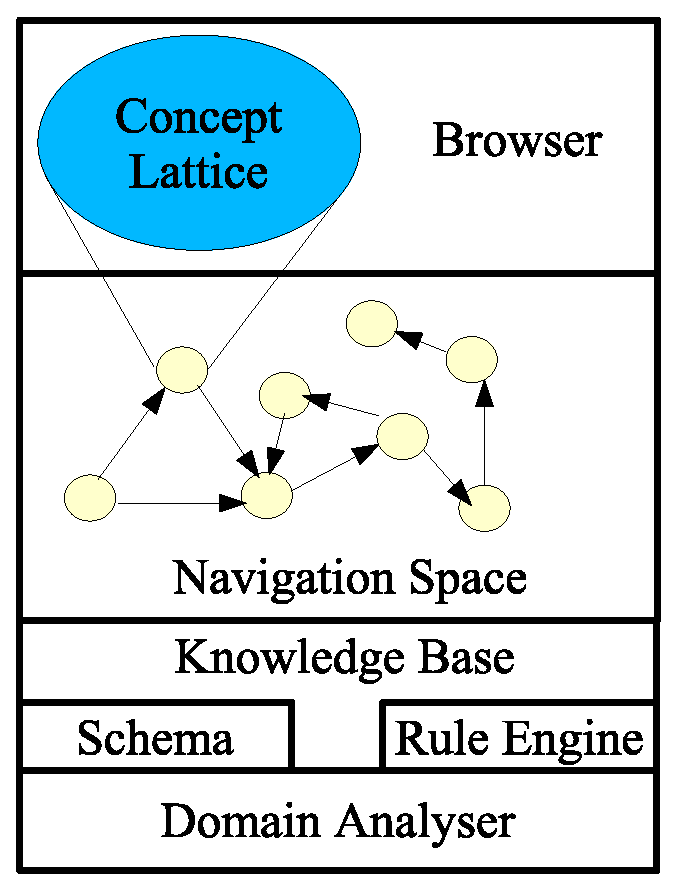
\includegraphics[height=0.8 \textheight]{img/system1.eps}
 % system1.eps: 1179666x1179666 pixel, 300dpi, 9987.84x9987.84 cm, bb=0 0 310 412
\end{center}
\end{slide}

\overlays{4}{
\begin{slide}{Bits and pieces}
\begin{itemstep}
 \item Jena as RDF storage and query engine
 \item Eclipse for extracting the source code structure
 \item Tupleware as FCA visualisation tool
 \item Crepe as CG editor
\end{itemstep}
\end{slide}
}

\overlays{4}{
\begin{slide}{Jena}
\begin{itemstep}
 \item Jena is an Java library for storing, manipulating and querying RDF
 \item It was originally developed by Hewlett Packard
 \item It is available as OSS project on Sourceforge
 \item It has been around for a long time
\end{itemstep}
\end{slide}
}

\overlays{4}{
\begin{slide}{Eclipse}
\begin{itemstep}
 \item Eclipse is best known as Java IDE
 \item It is a large framework consisting of many different plugins
 \item The strong emphasis on plugins makes it easy to extend
 \item The Java Development Tools (JDT) offer access to a combination
       of AST and DOM
\end{itemstep}
\end{slide}
}

\overlays{5}{
\begin{slide}{Tupleware}
\begin{itemstep}
 \item Tupleware is a fork of the ToscanaJ project
 \item It generates Hasse diagrams using the ToscanaJ components
 \item The approach of creating the diagrams is rather different
 \begin{itemstep}
  \item ToscanaJ uses Conceptual Scaling
  \item Tupleware uses relational algebra
 \end{itemstep}
\end{itemstep}
\end{slide}
}

\overlays{3}{
\begin{slide}{Crepe}
\begin{itemstep}
 \item Crepe is a prototypical CG editor
 \item It uses the graphical display form
 \item It was designed to study how strong schema support
       can make formal statement design easier
\end{itemstep}
\end{slide}
}

\part{Demo}

% TJ code, revision and size info, storyline

% Example: dependencies of toplevel packages
% Example: some more complex hierarchy

\part{Navigation Spaces}

\begin{slide}{Navigation Spaces}
 \begin{center}
  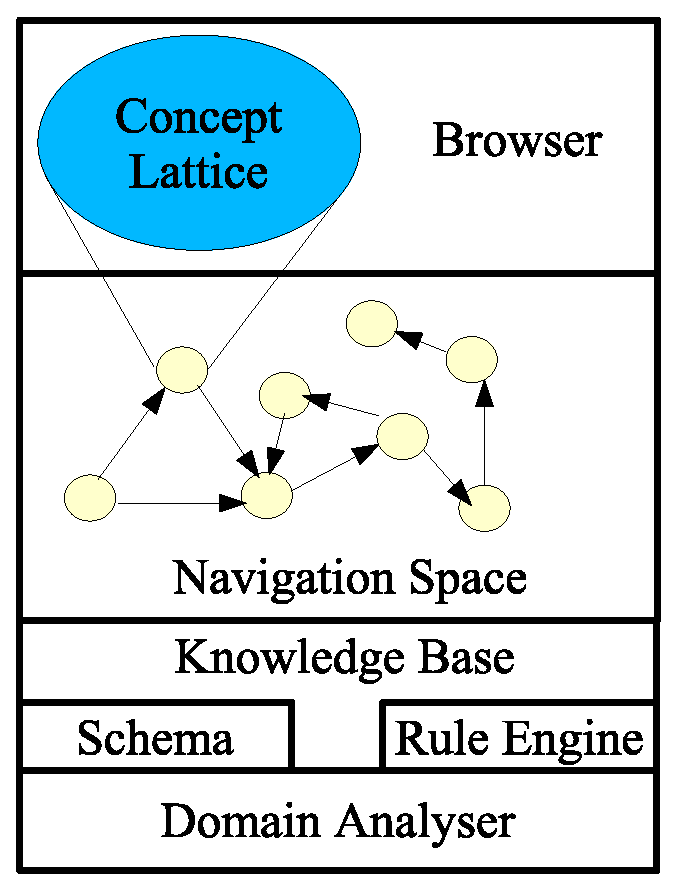
\includegraphics[height=0.8 \textheight]{img/system1.eps}
 \end{center}
\end{slide}

\begin{slide}{Navigation Spaces: toplevel}
 \begin{center}
  \includegraphics[height=0.8 \textheight]{img/callgraph-1.eps}
 \end{center}
\end{slide}

\begin{slide}{Navigation Spaces: focus}
 \begin{center}
  
\includegraphics[height=0.3 \textheight]{img/callgraph-2.eps}
 \end{center}
\end{slide}

\begin{slide}{Navigation Spaces: expand}
 \begin{center}
  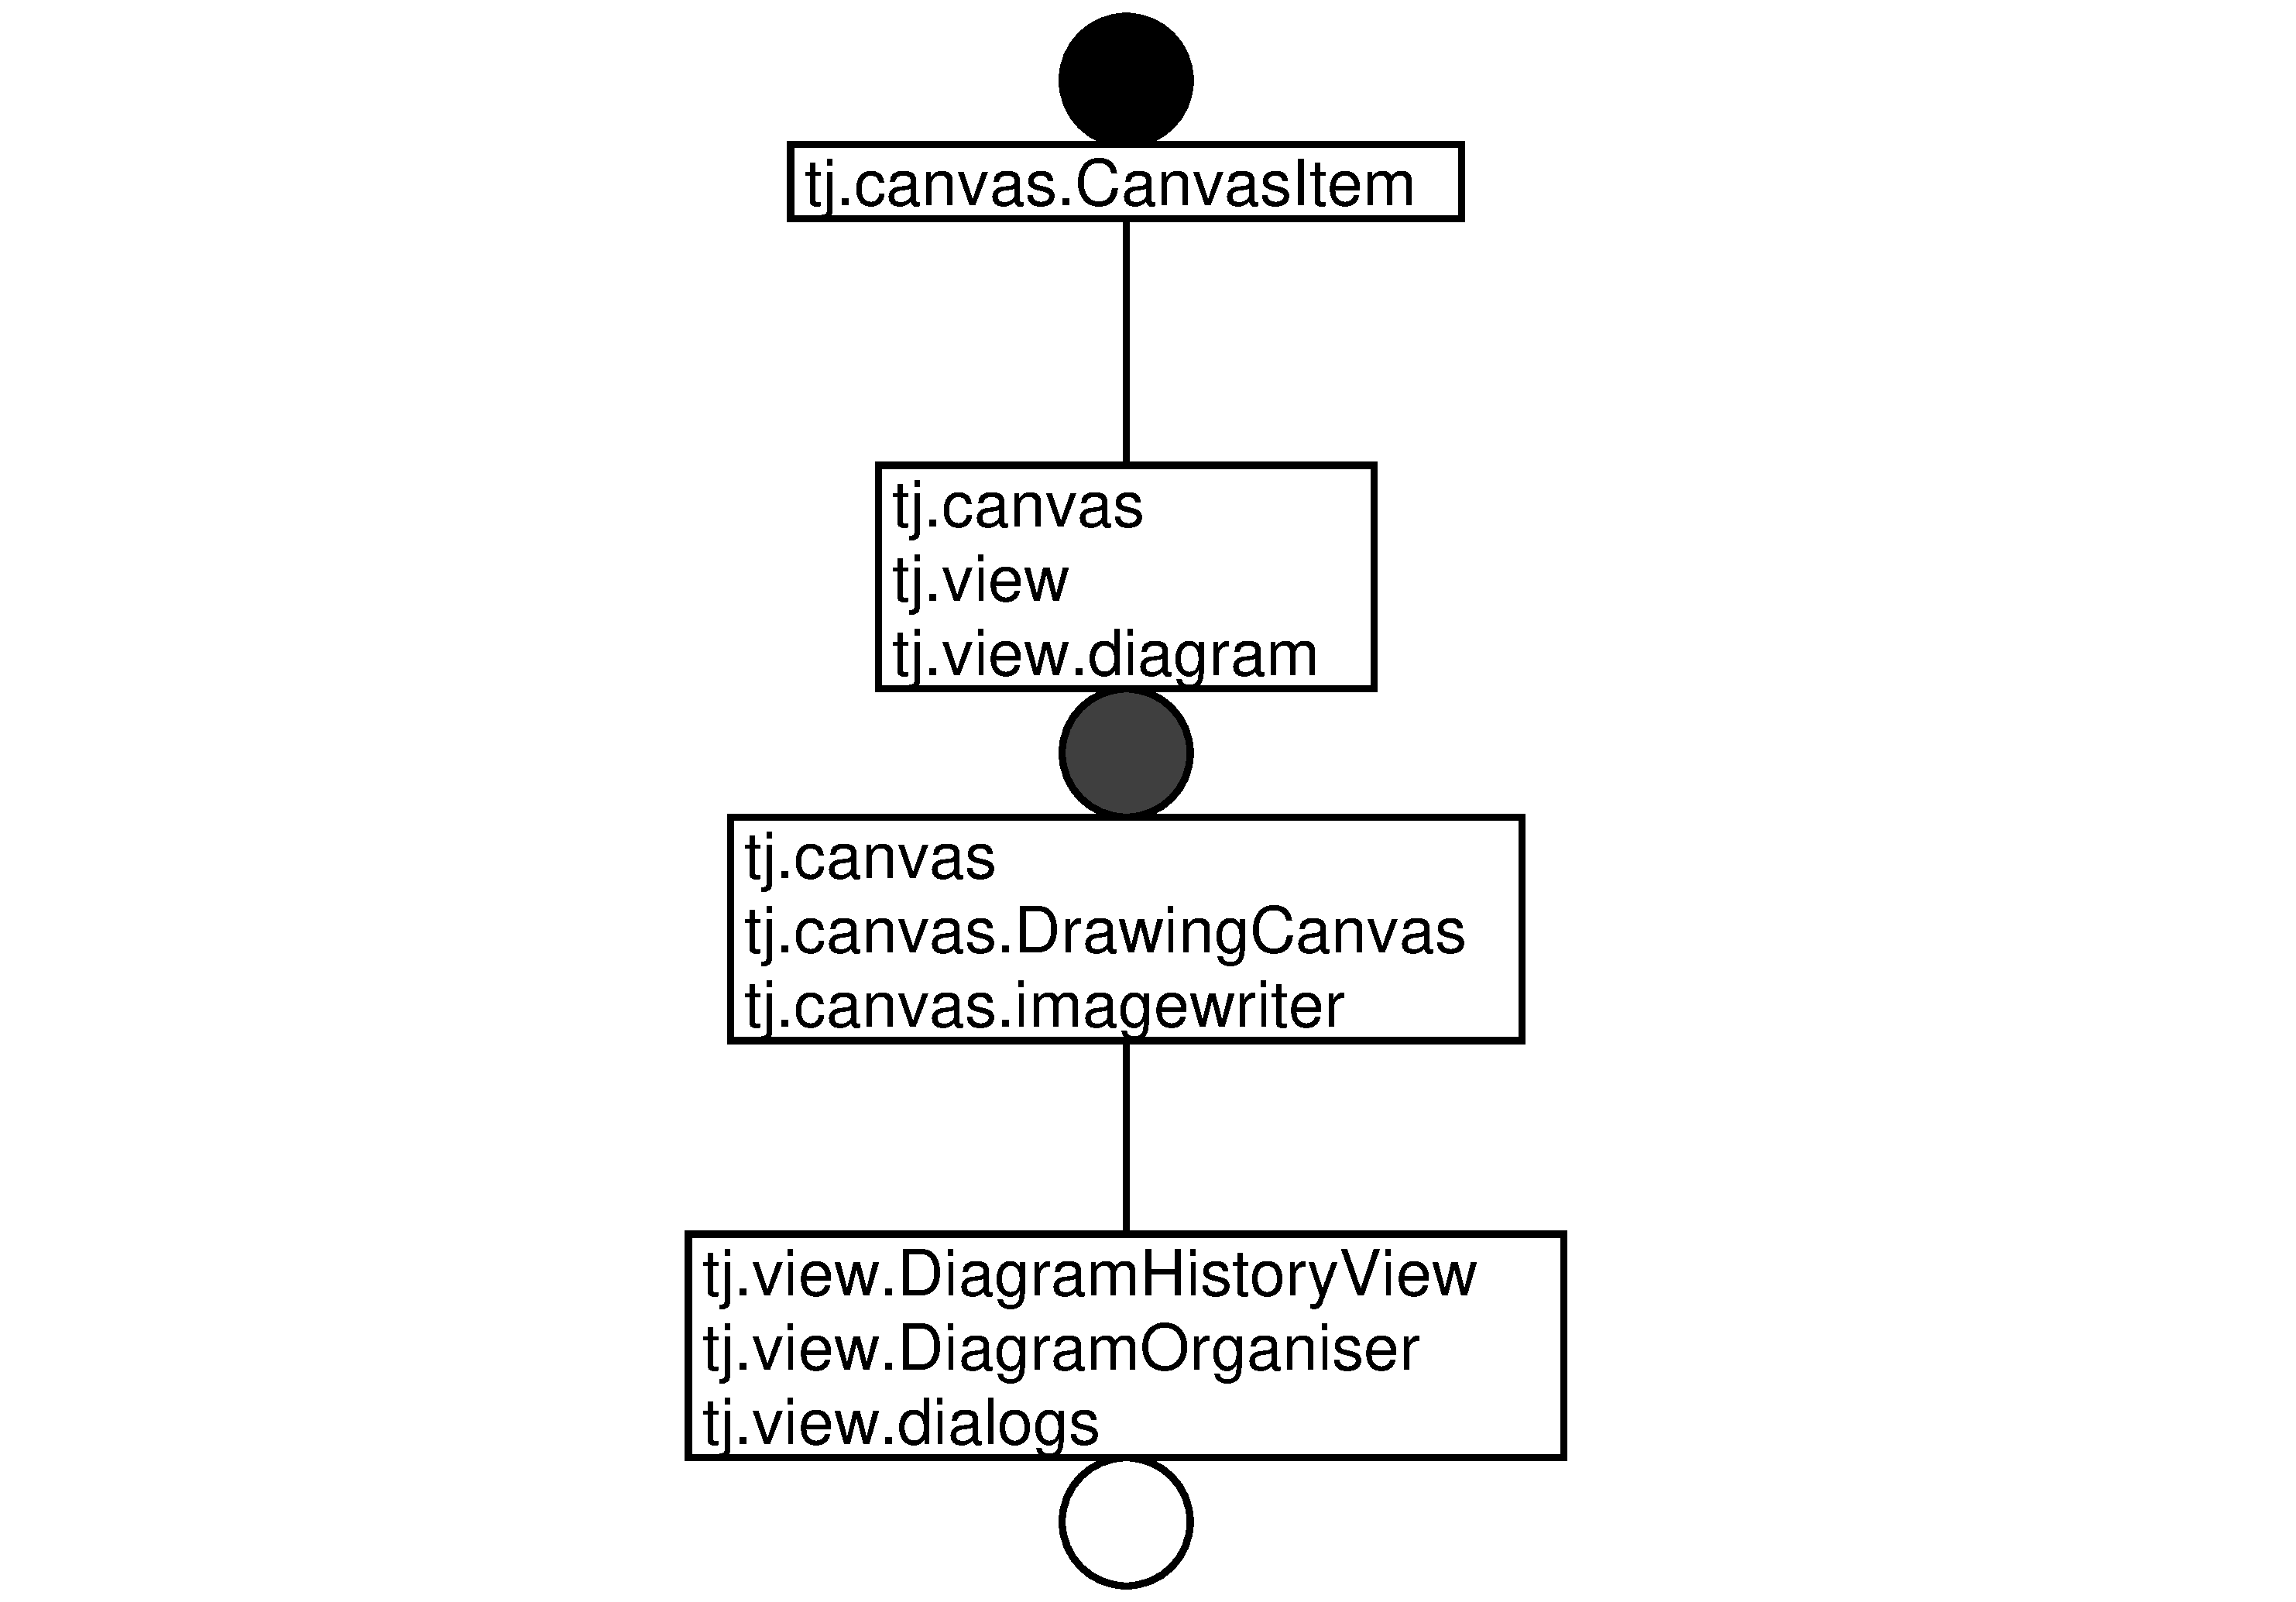
\includegraphics[height=0.8 \textheight]{img/callgraph-3.eps}
 \end{center}
\end{slide}

\begin{slide}{Navigation Spaces: expand}
 \begin{center}
  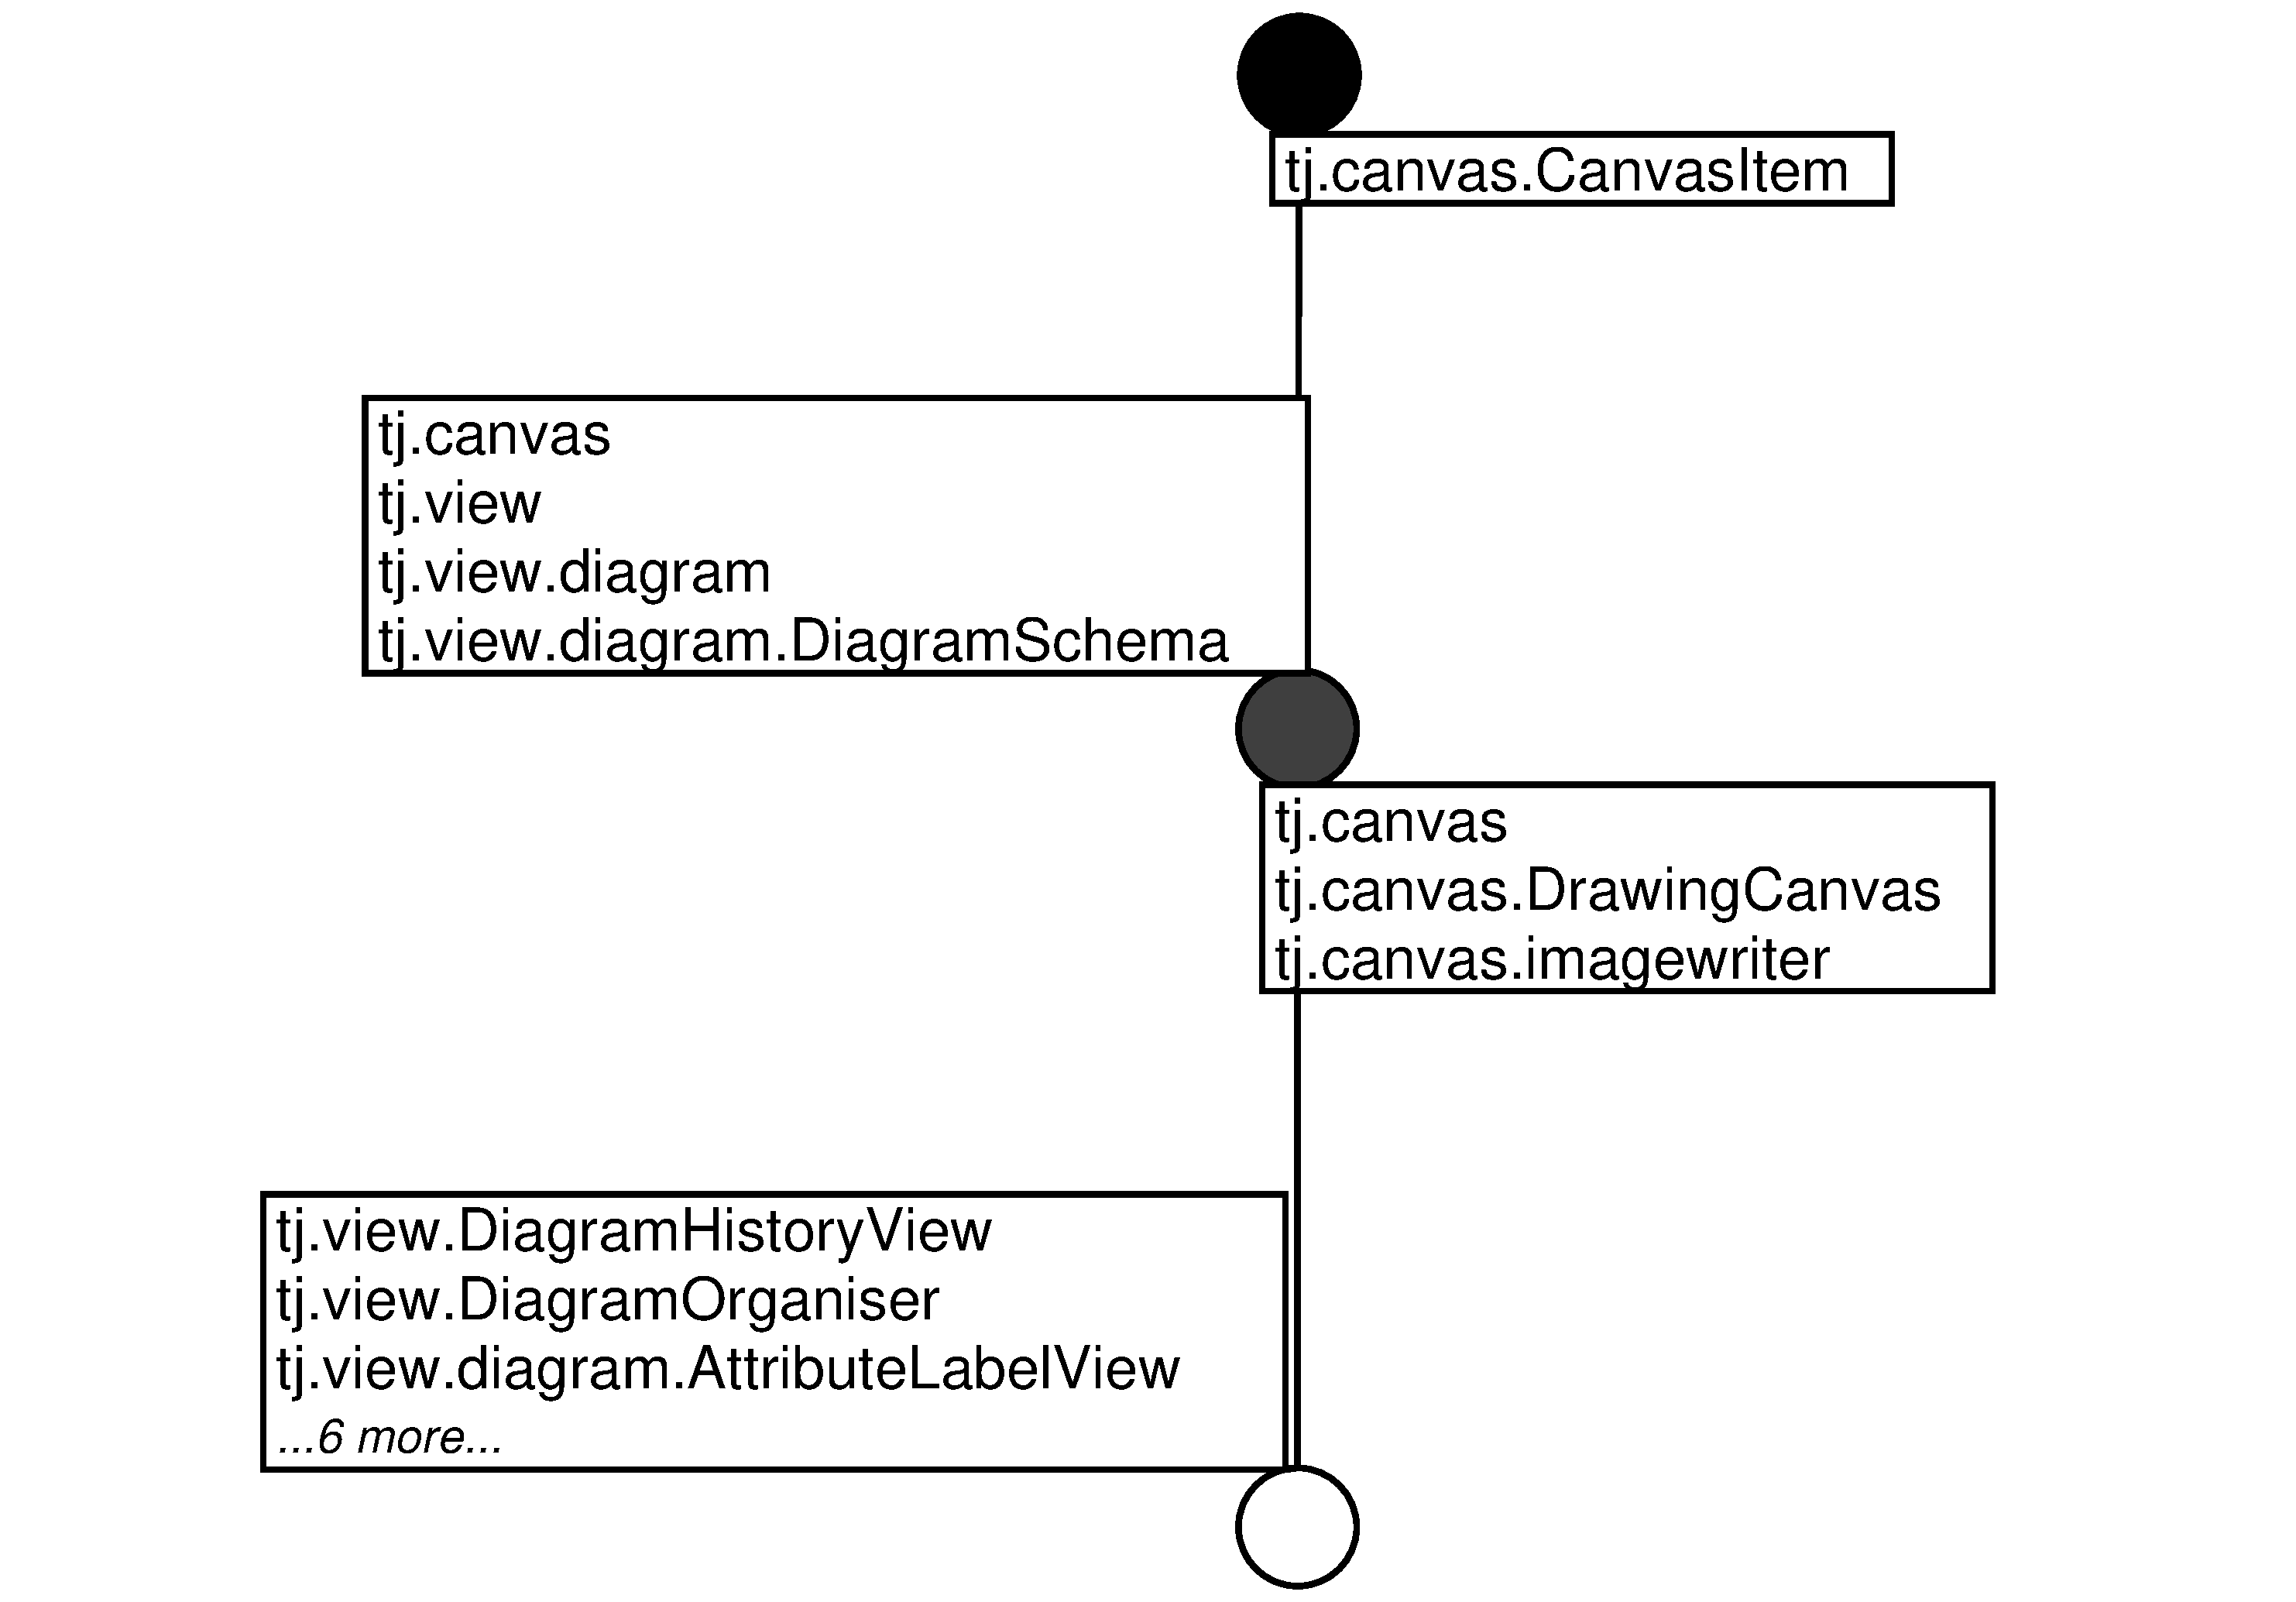
\includegraphics[height=0.8 \textheight]{img/callgraph-4.eps}
 \end{center}
\end{slide}

\begin{slide}{Navigation Spaces: expand}
 \begin{center}
  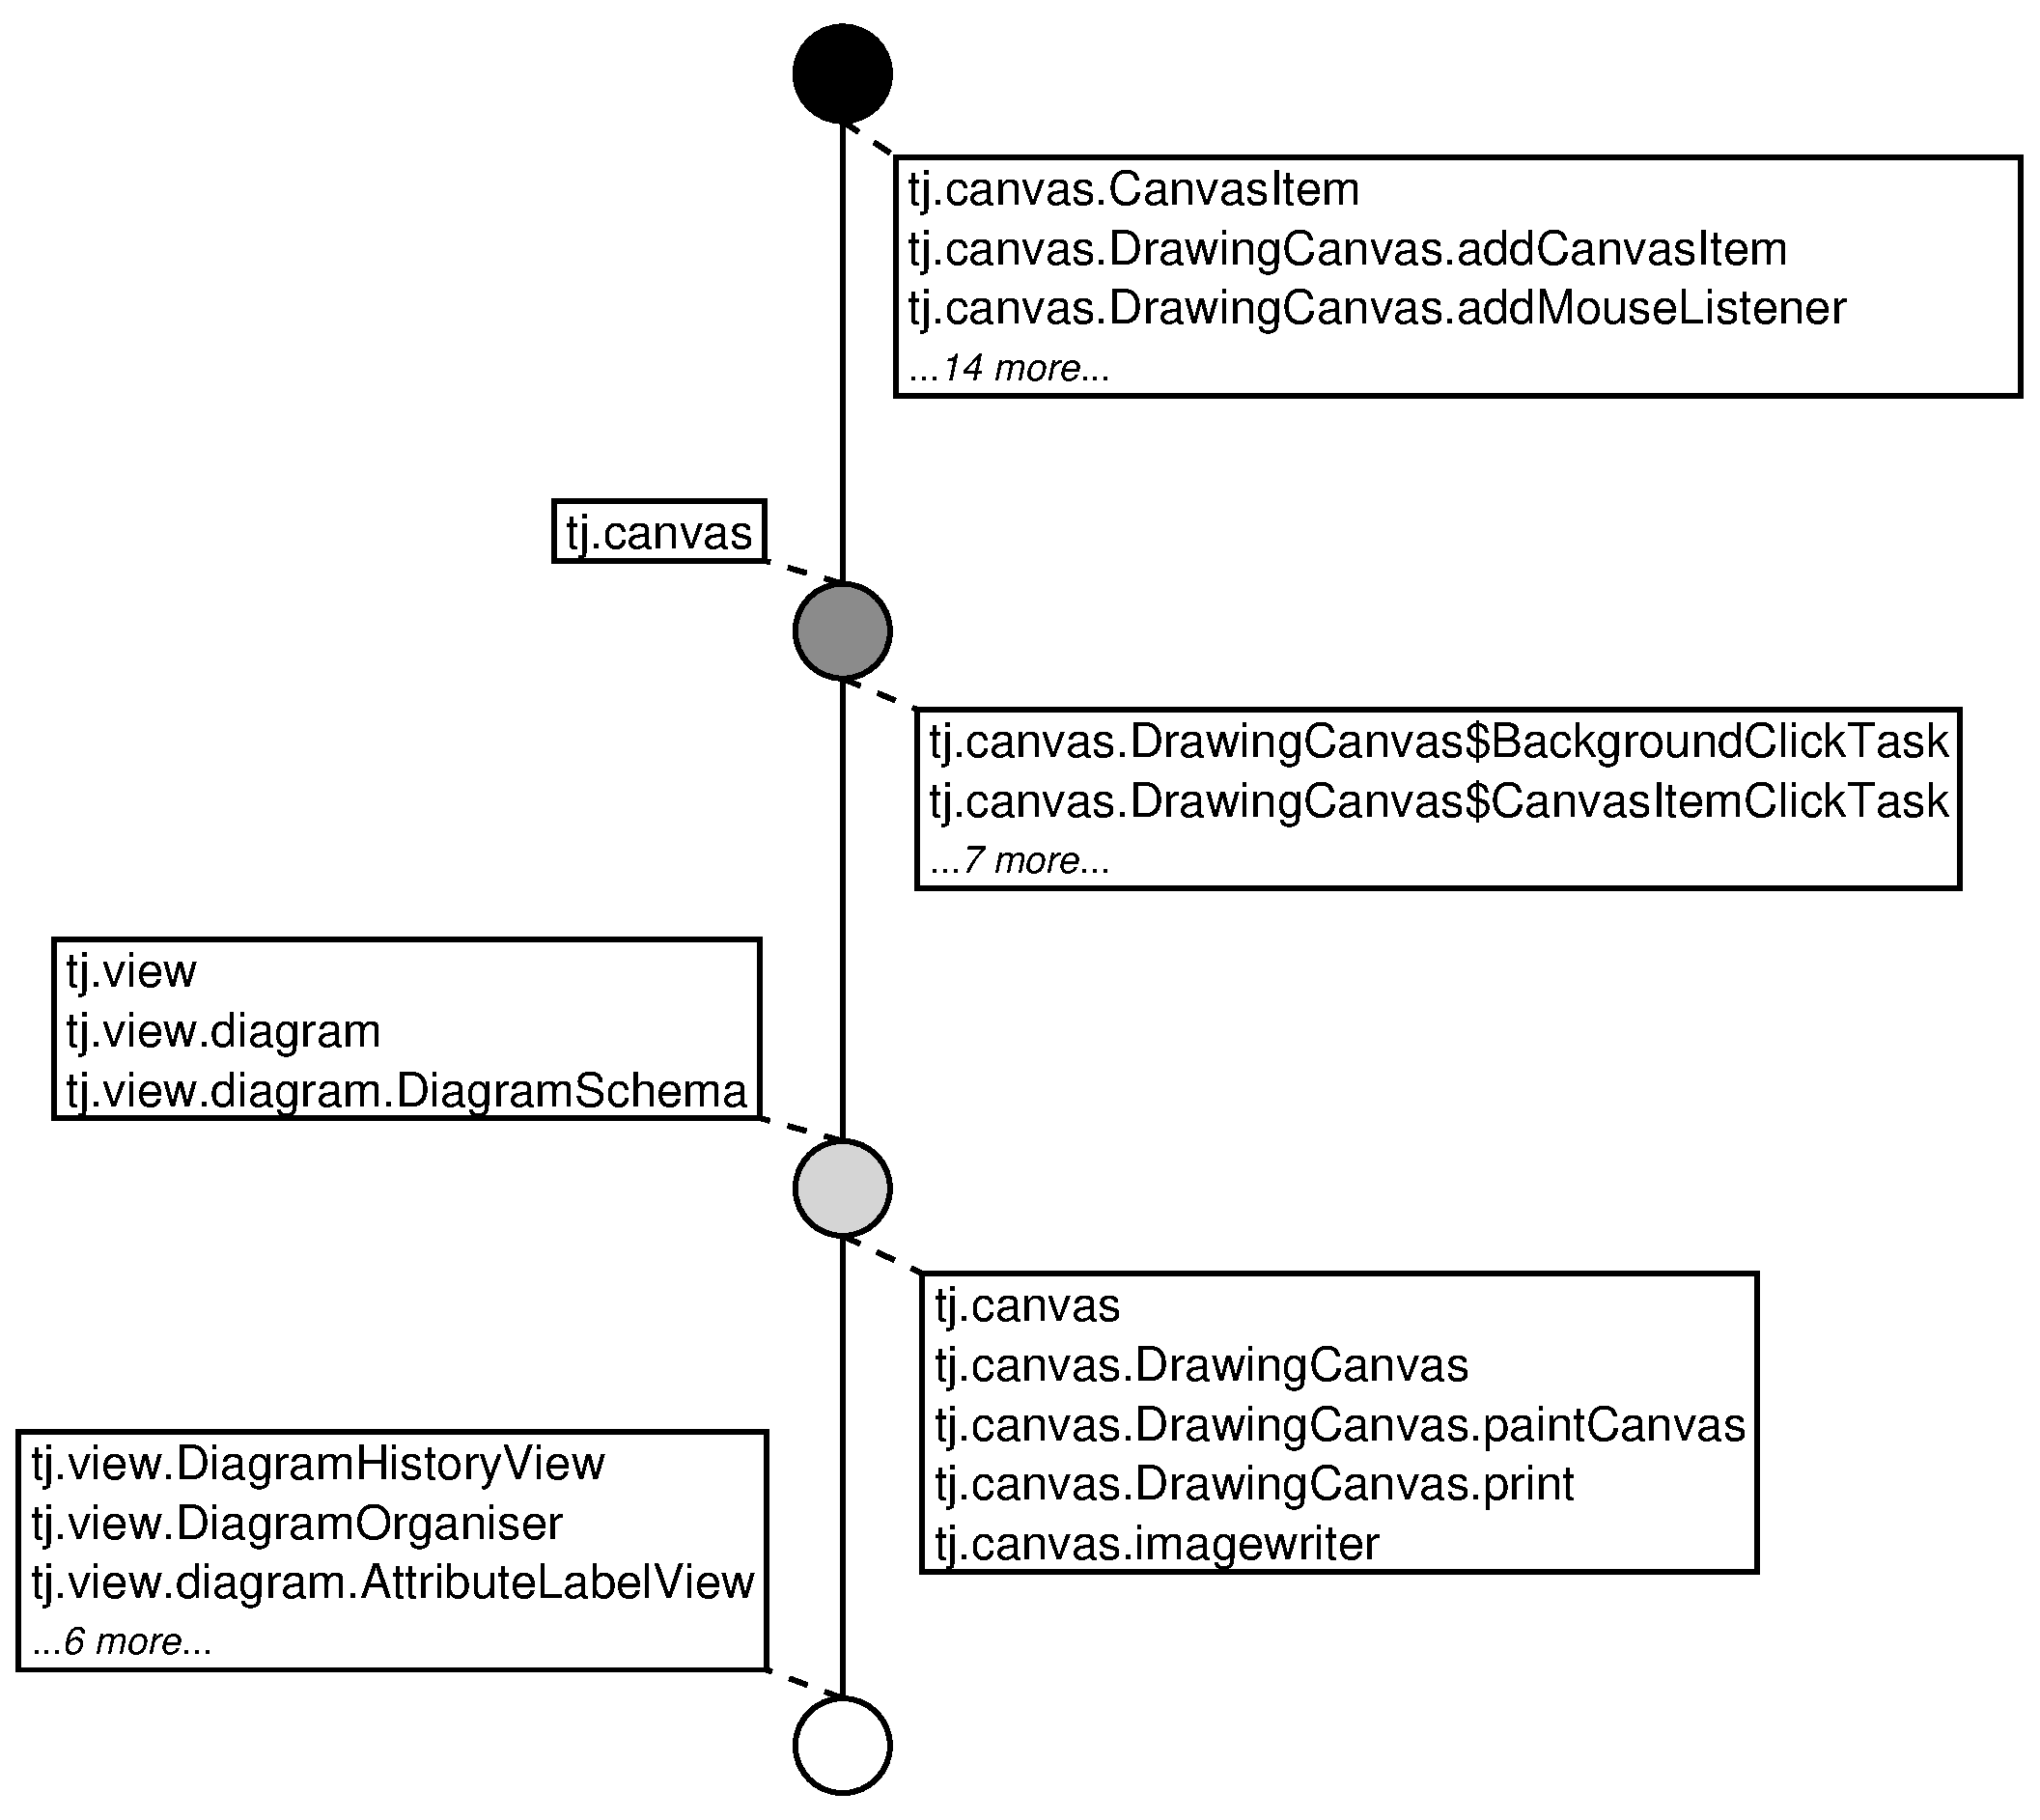
\includegraphics[height=0.8 \textheight]{img/callgraph-5.eps}
 \end{center}
\end{slide}

\begin{slide}{Navigation Spaces: go to source}
 \begin{center}
  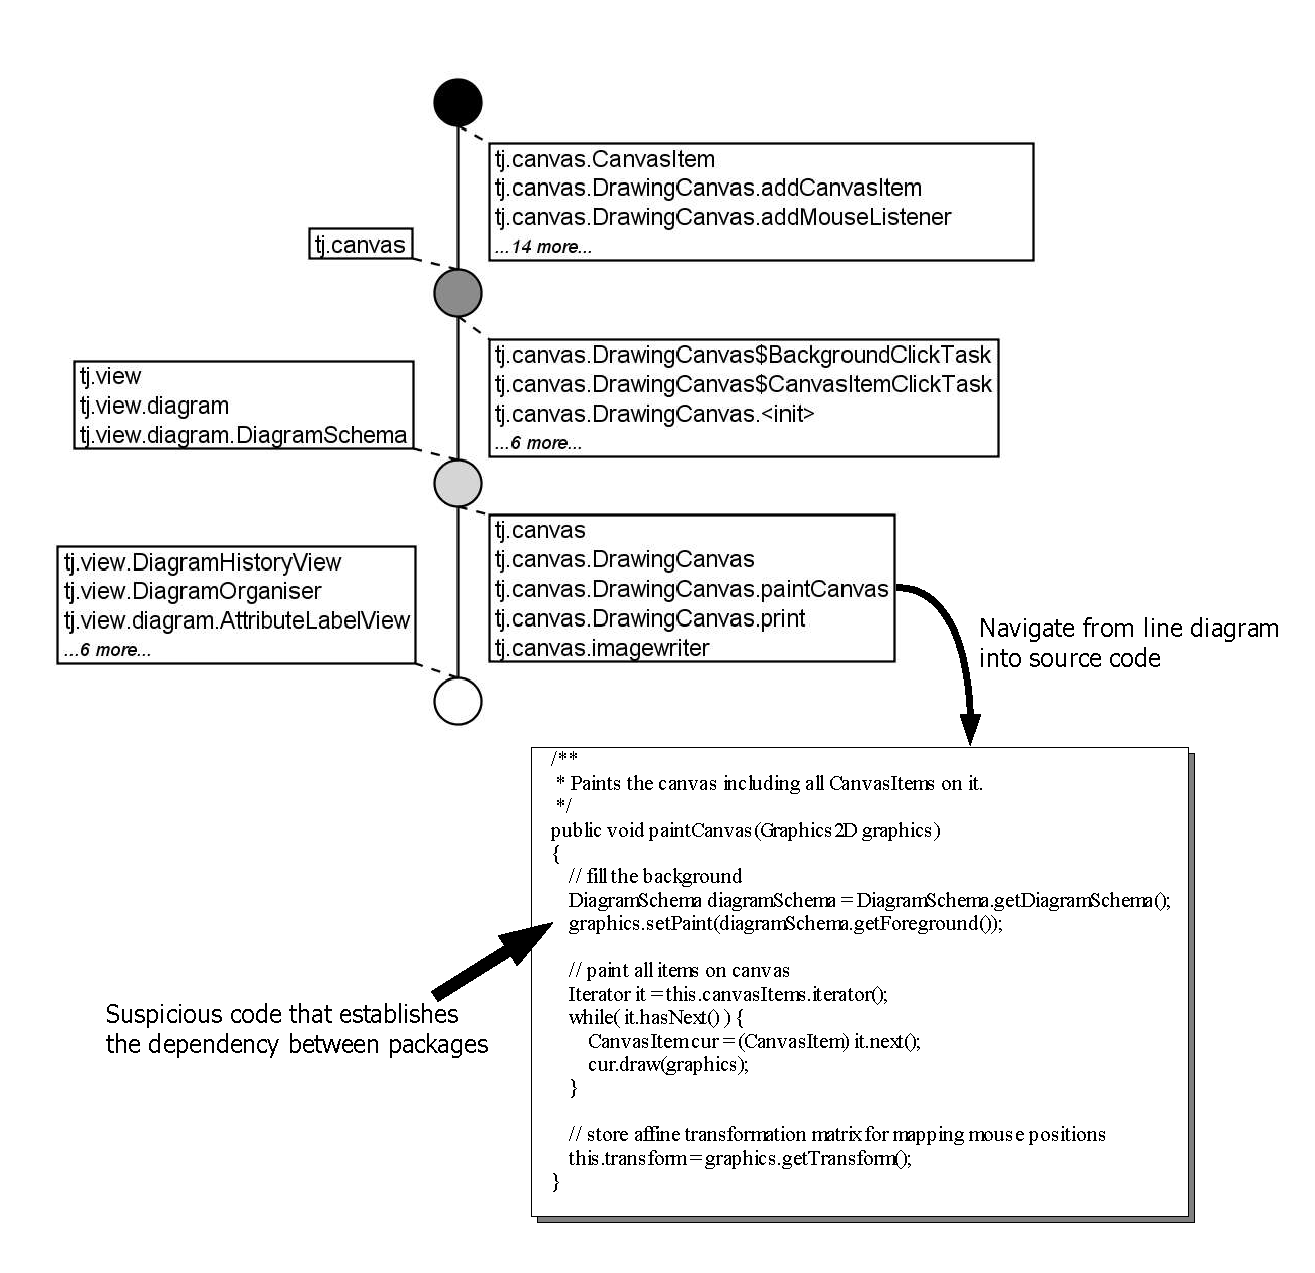
\includegraphics[height=0.8 \textheight]{img/sourceNavigation.eps}
 \end{center}
\end{slide}

\part{Structural Decomposition}

\overlays{4}{
\begin{slide}{Structural Decomposition}
\begin{itemstep}
 \item Many structures found can be decomposed into a set of simpler structures
 \item Horizontal decomposition just splits into two parts that connect only
       at the top and bottom of the lattice
 \item More interesting is usually factorization: explain a larger structure
       by considering it as a product of two independent factors
 \item This is not just coincidentally related to ``refactoring''
\end{itemstep}
\end{slide}
}

\overlays{2}{
\begin{slide}{Structural Decomposition: STL container classes}
 \onlySlide*{1}{%
  \begin{center}
   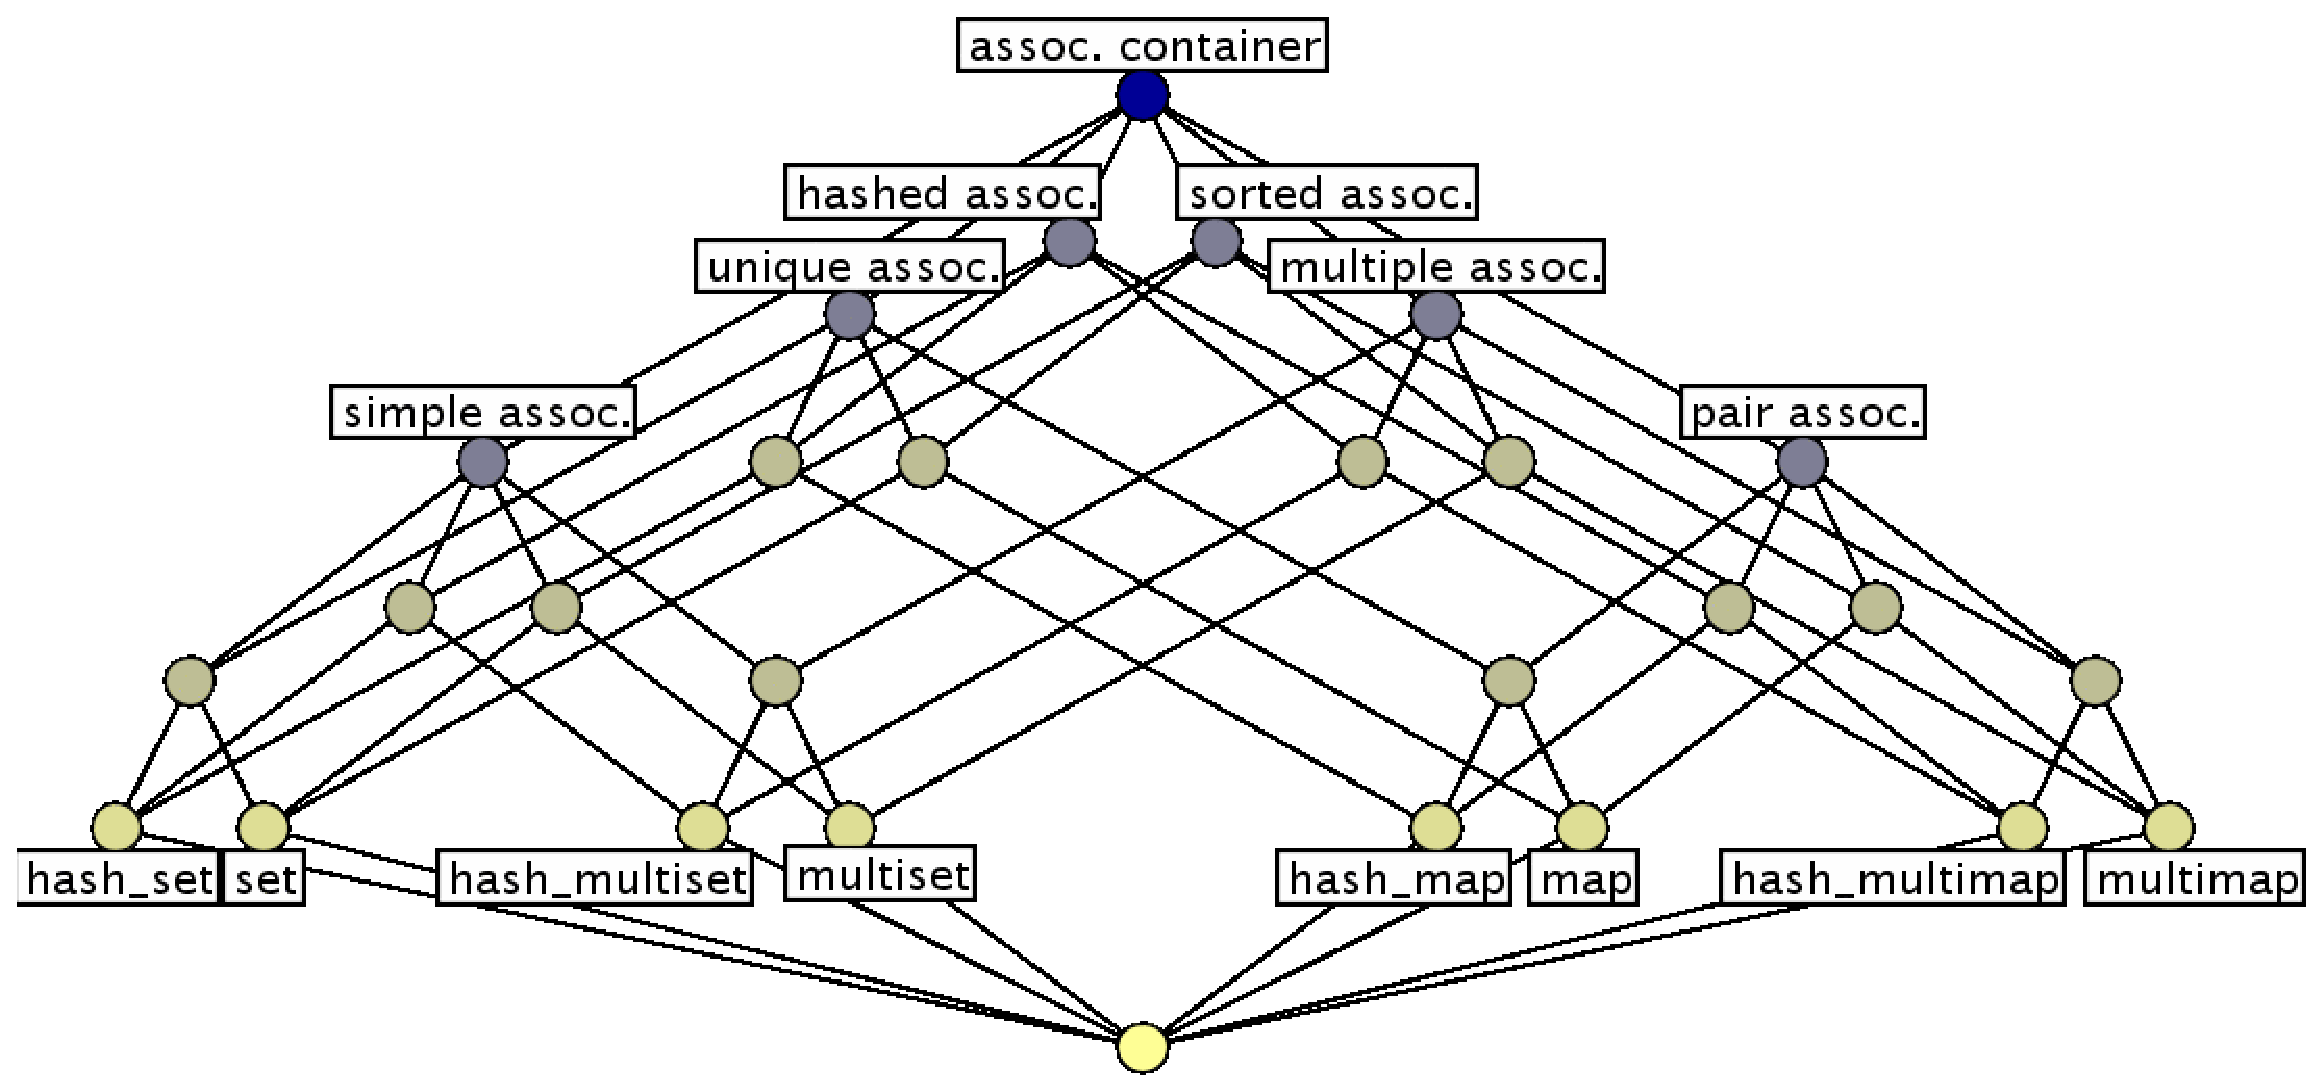
\includegraphics[height=0.5 \textheight]{img/stl.eps}
  \end{center}
 }%
 \onlySlide*{2}{%
  \begin{center}
   \includegraphics[height=0.6 \textheight]{img/stl_derived.eps}
  \end{center}
 }%
\end{slide}
}

\overlays{5}{
\begin{slide}{Decomposing the STL classes}
 \begin{center}
 \fromSlide{1}{%
  \includegraphics*[width=0.8 \textwidth,viewport=0 100 1409 750,clip]{img/k1234.eps} \\
 }%
 \fromSlide{2}{%
  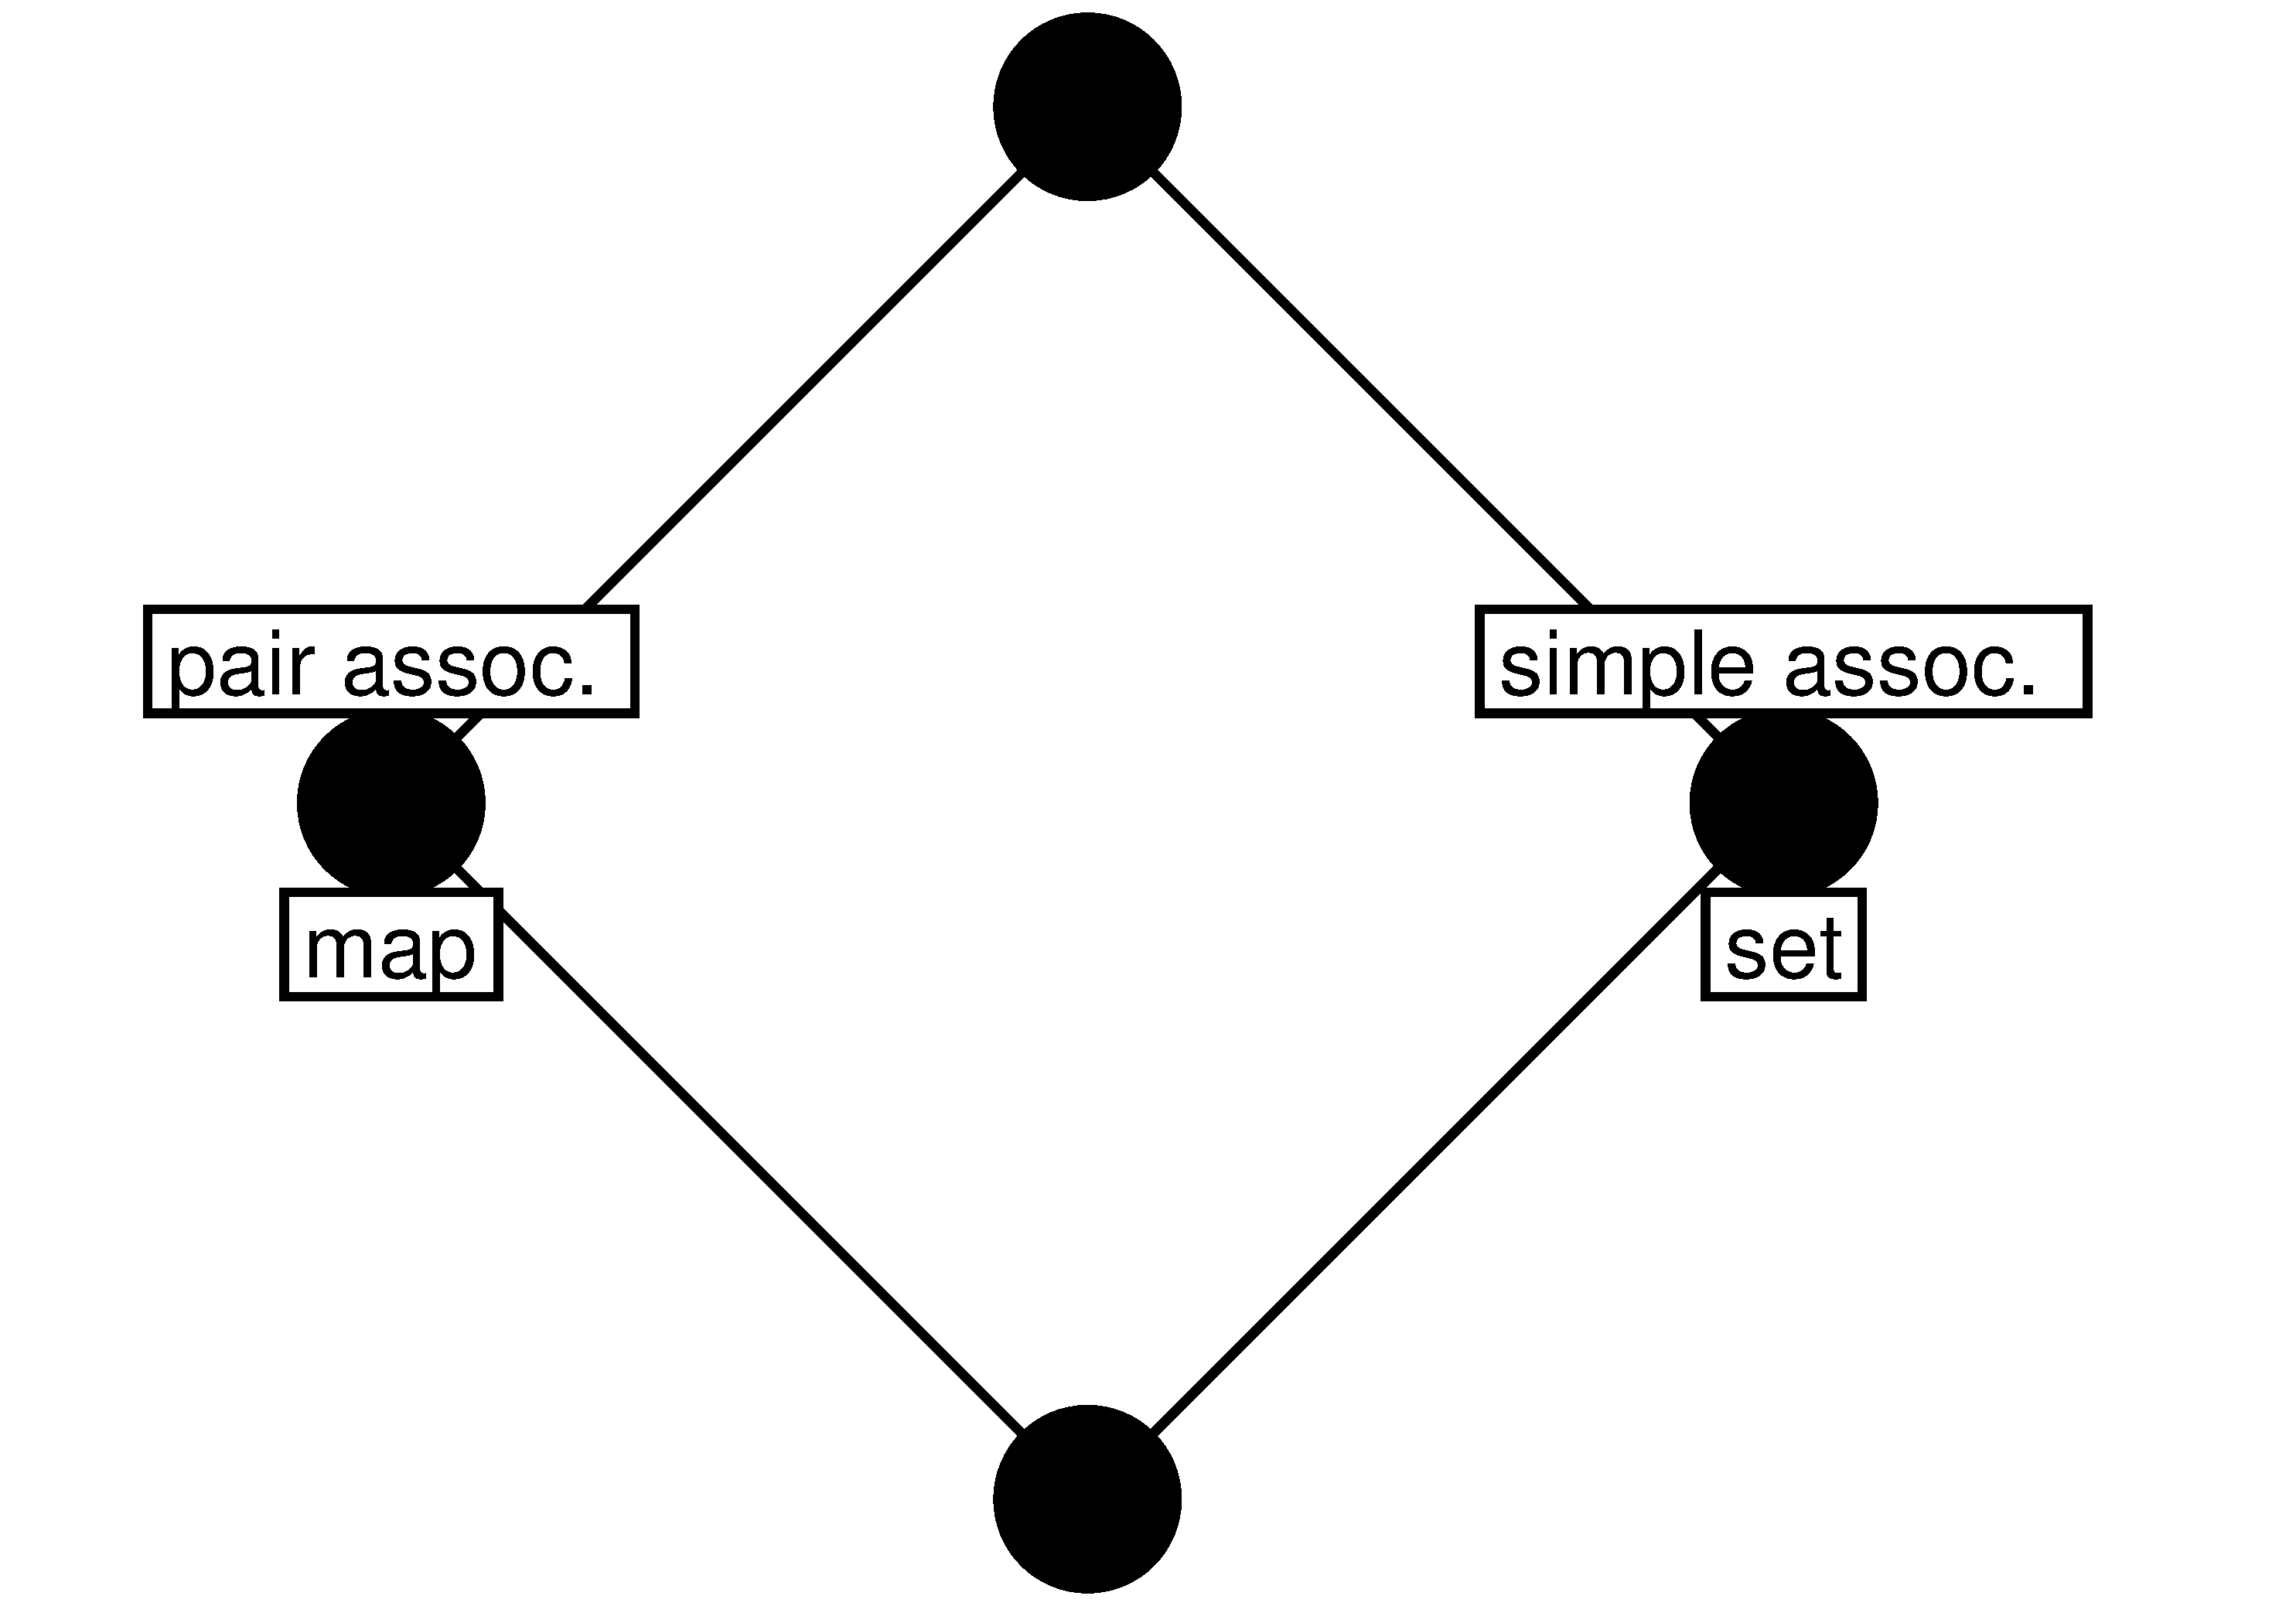
\includegraphics[width=0.23 \textwidth]{img/k2.eps}
 }%
 \fromSlide{3}{%
  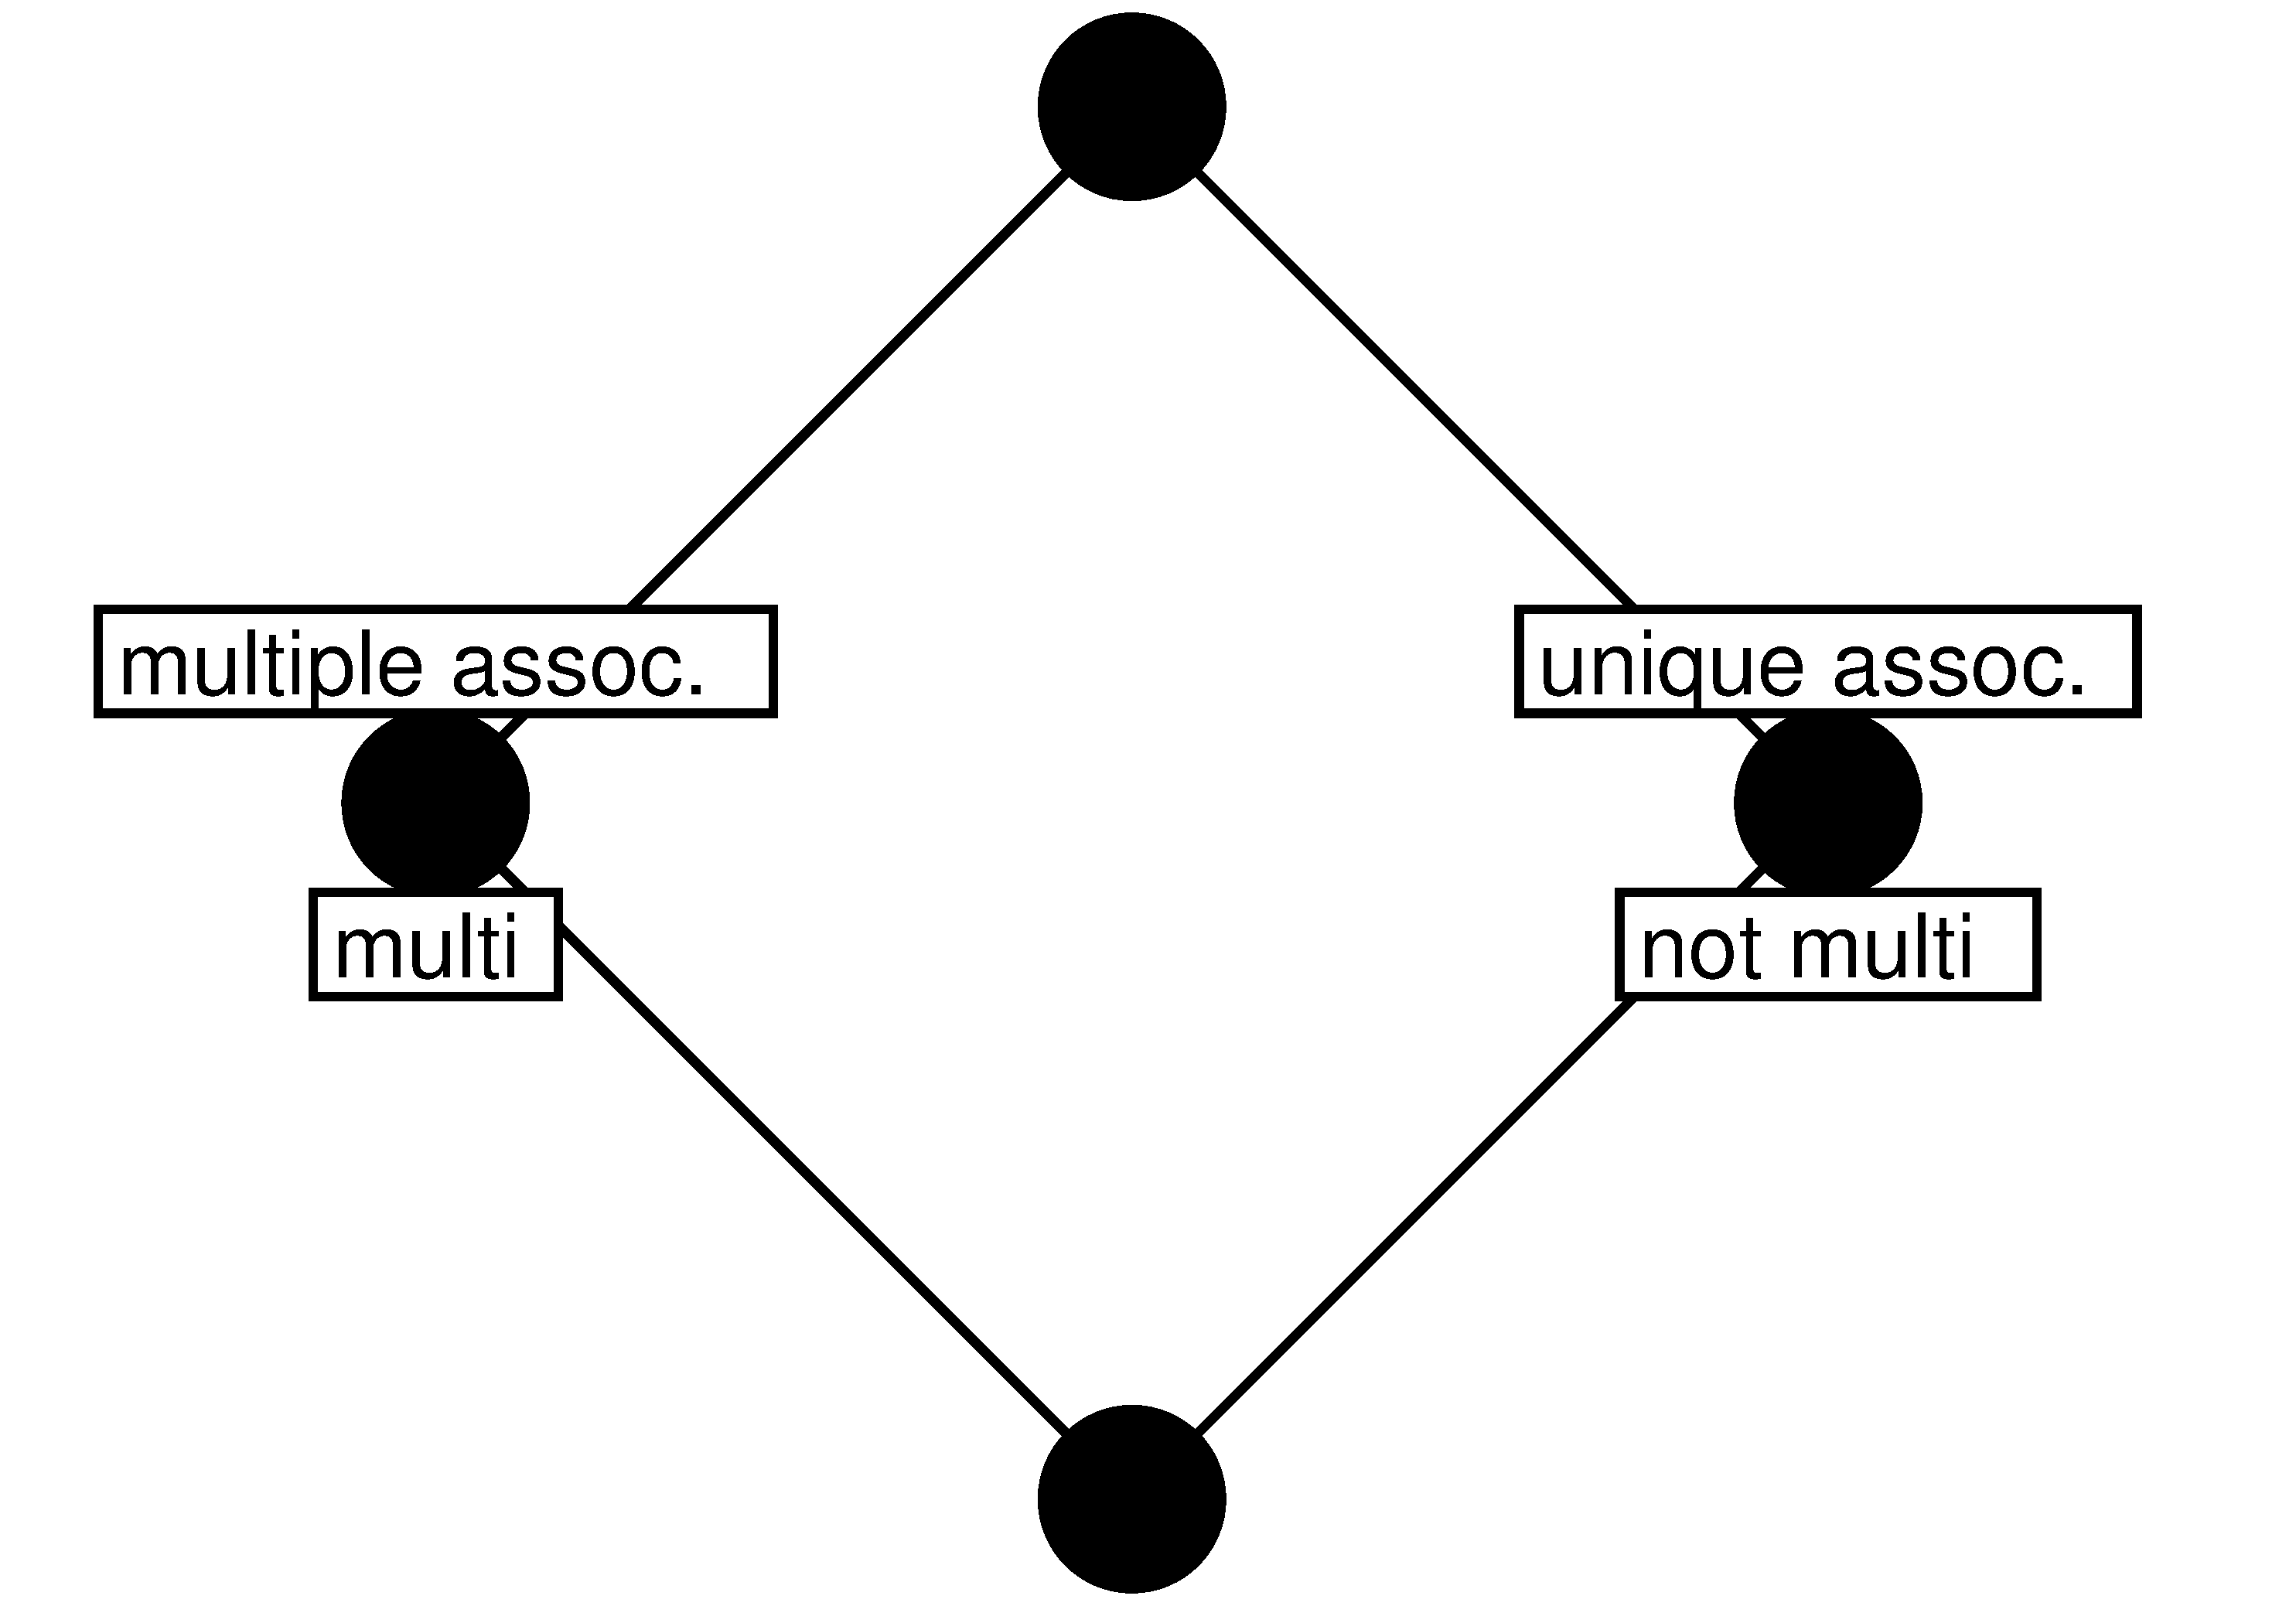
\includegraphics[width=0.23 \textwidth]{img/k3.eps}
 }%
 \fromSlide{4}{%
  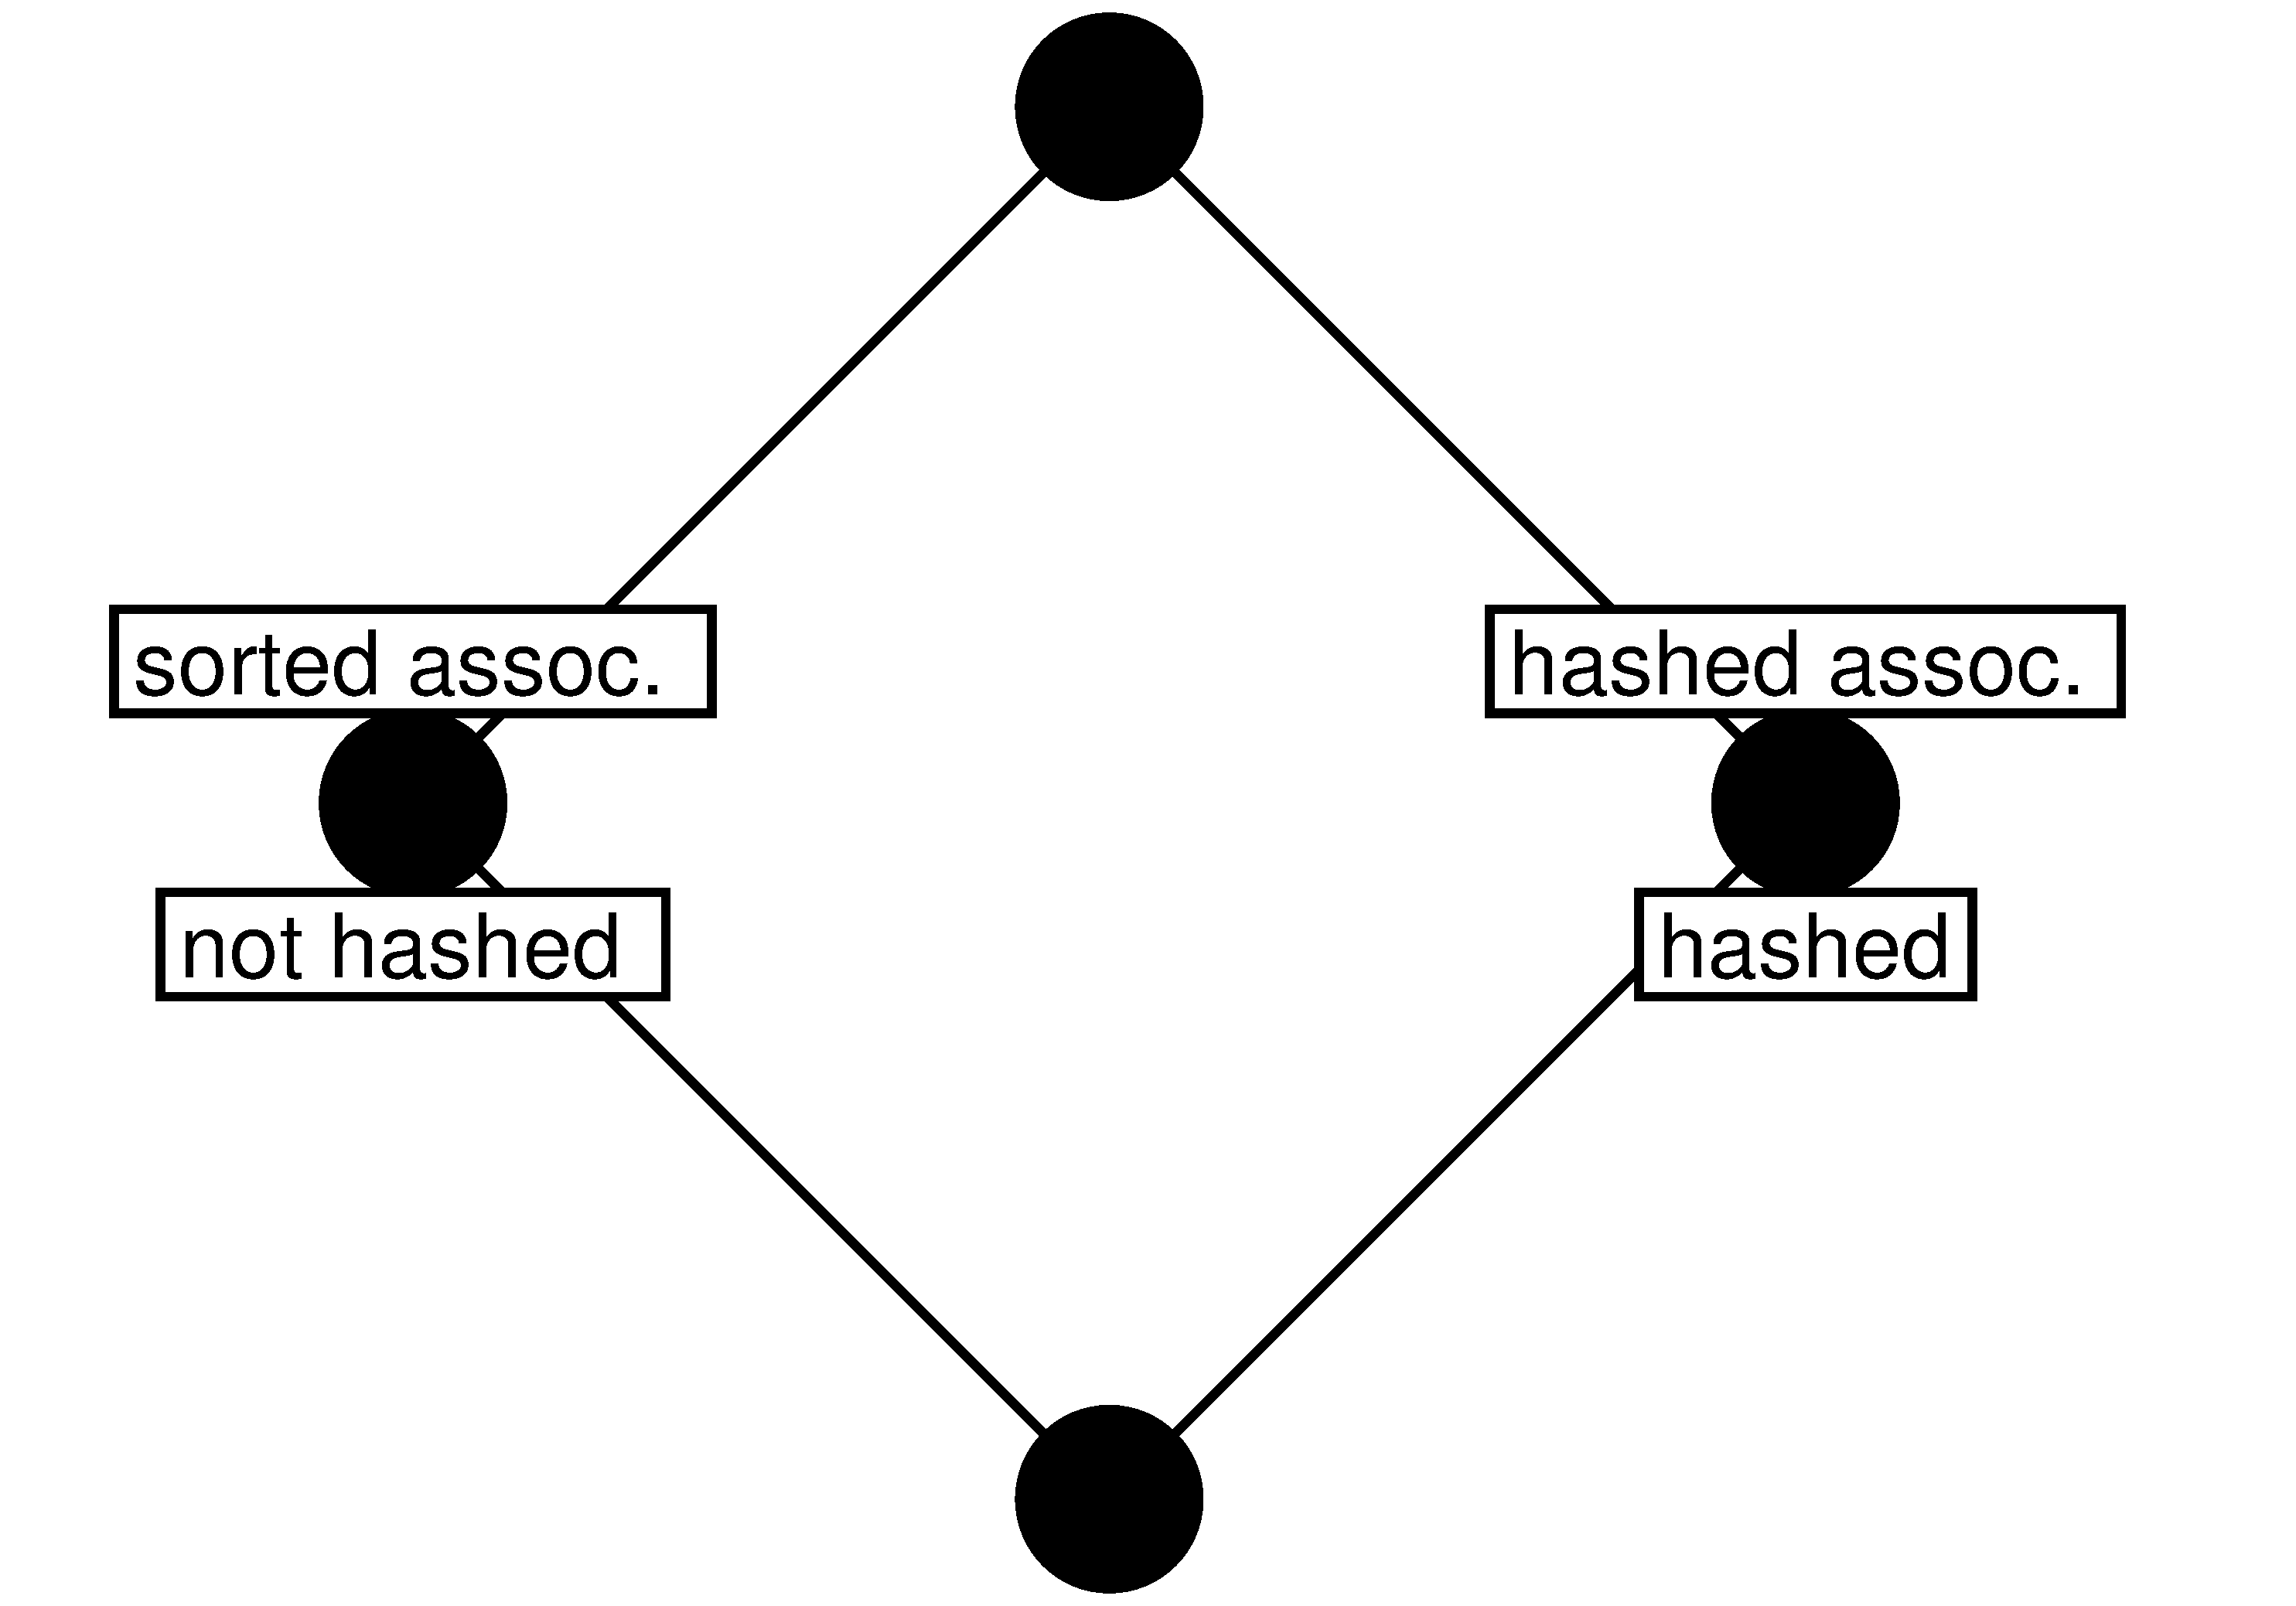
\includegraphics[width=0.23 \textwidth]{img/k4.eps}
 }%
 \fromSlide{5}{%
  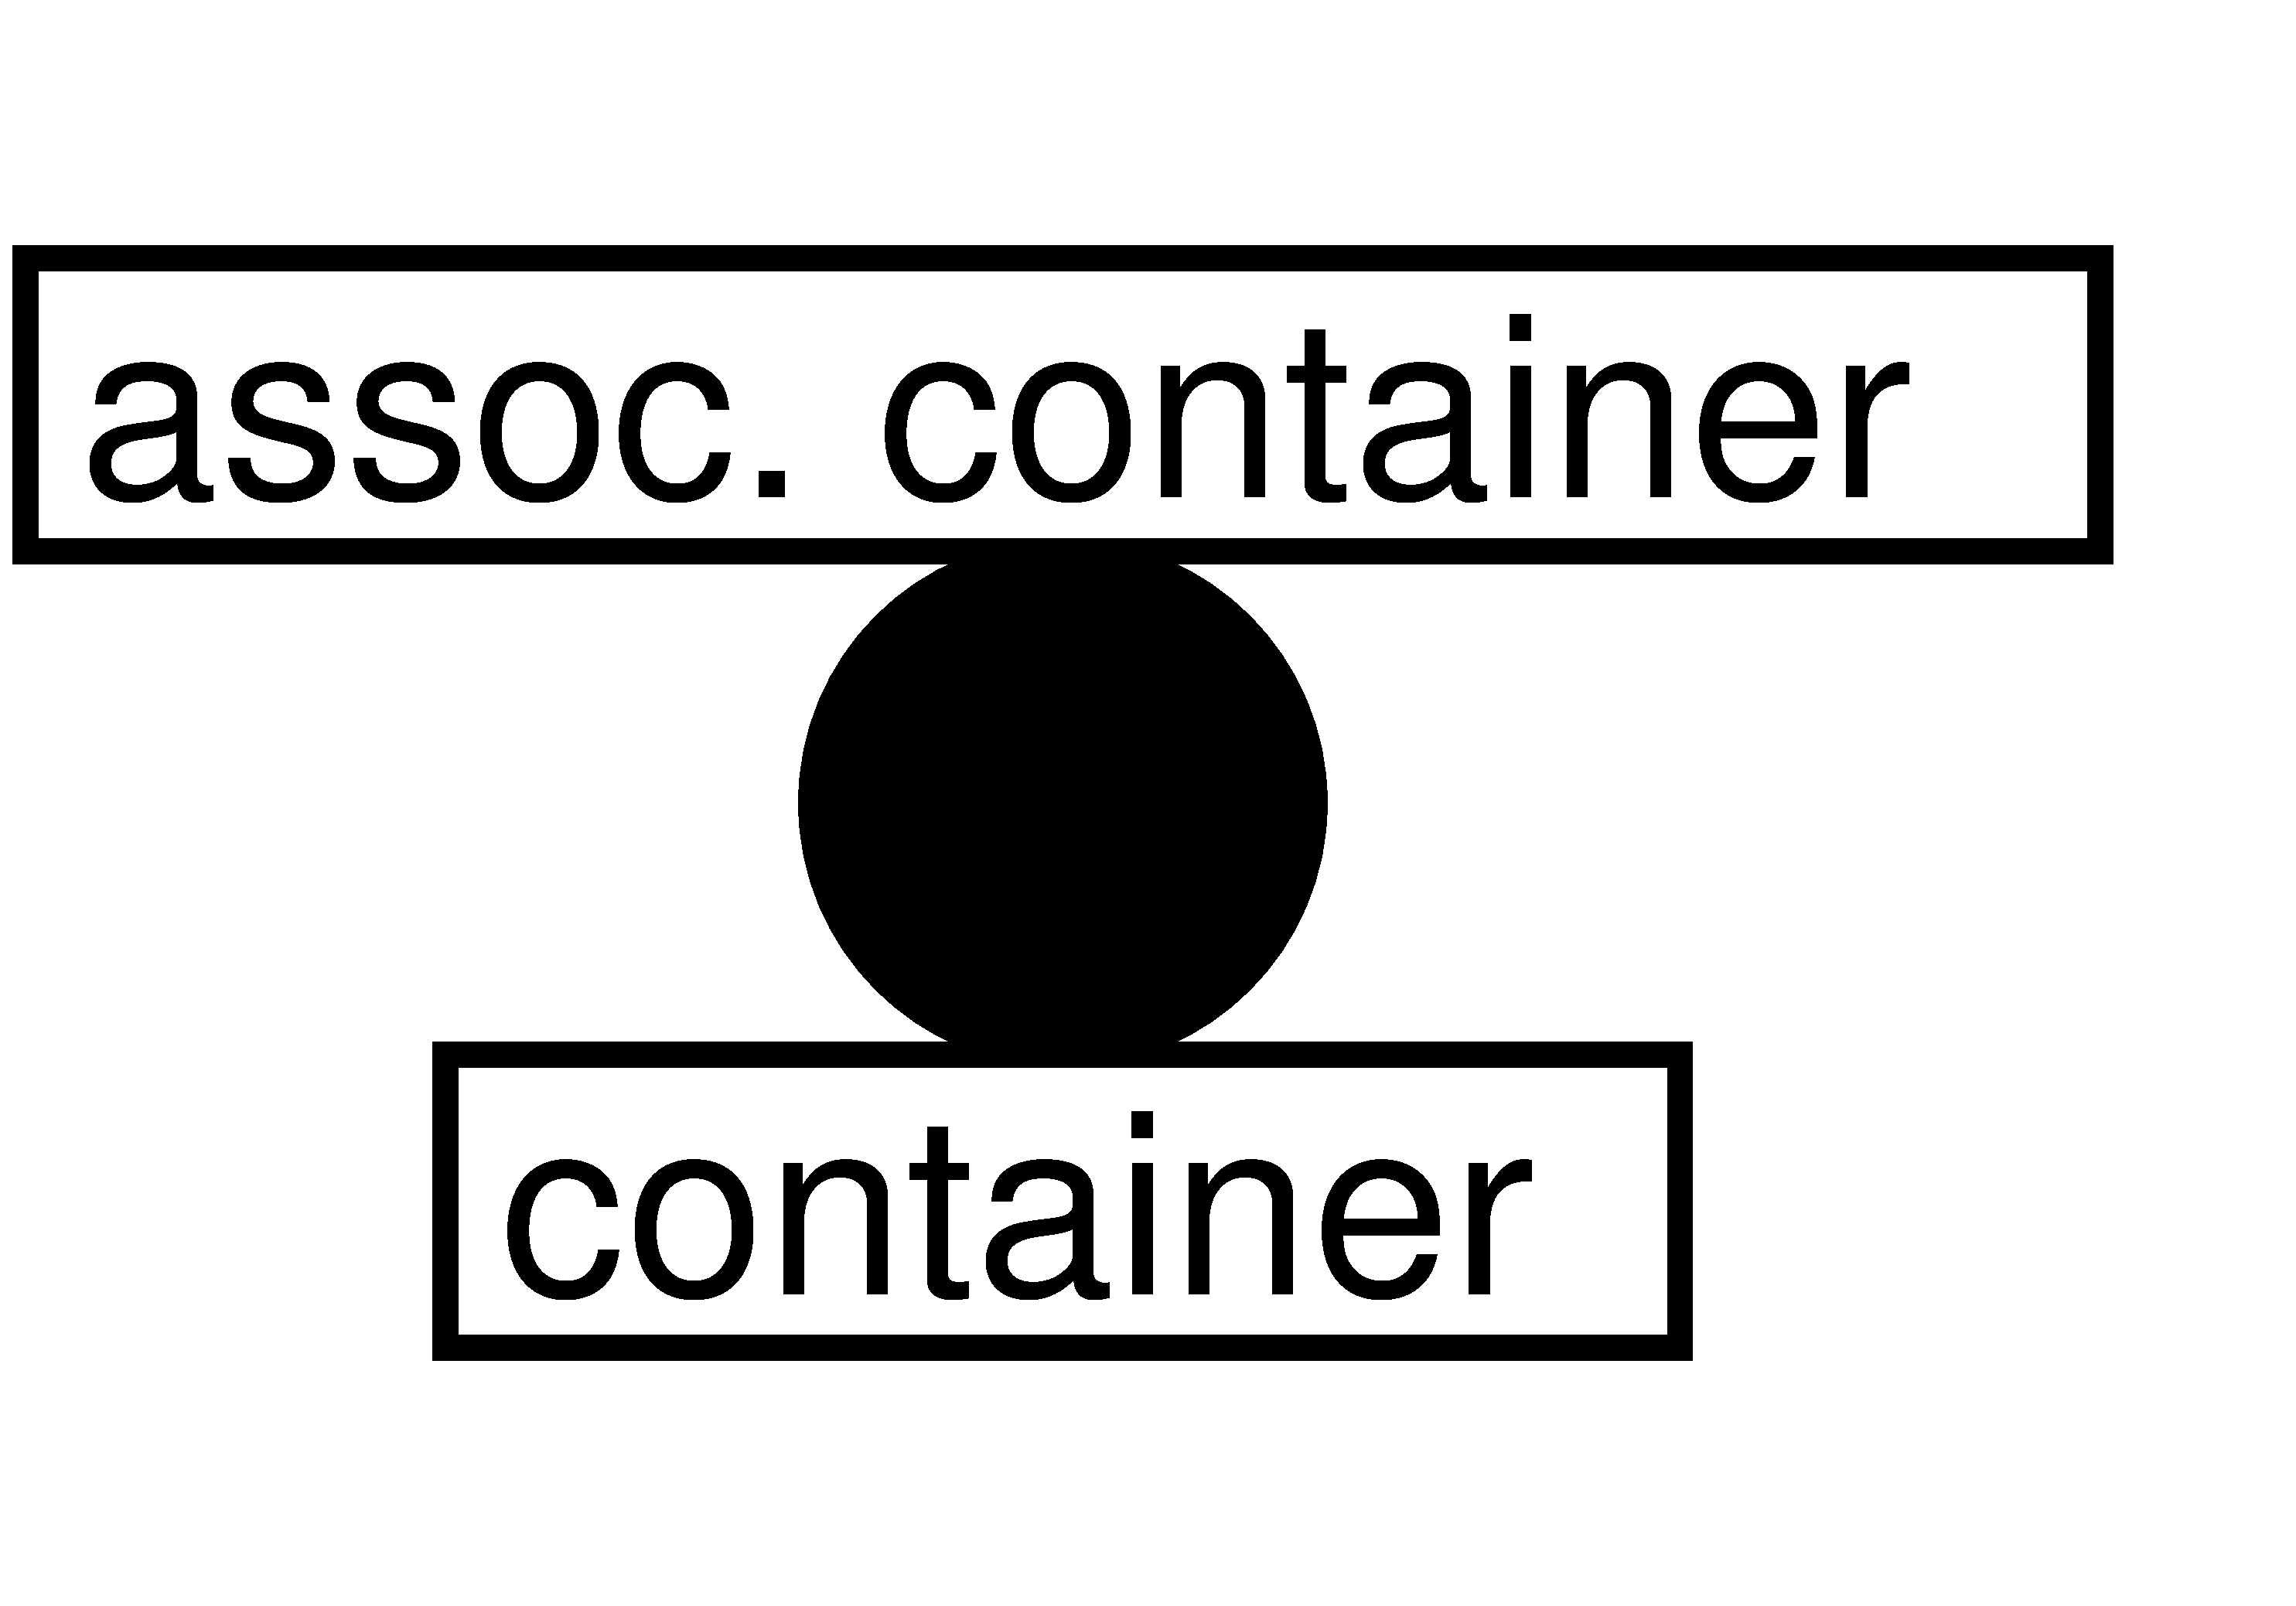
\includegraphics[width=0.1 \textwidth]{img/k1.eps}
 }%
 \end{center}
\end{slide}
}

\begin{slide}{Structural Decomposition: Java Collection API}
 \begin{center}
  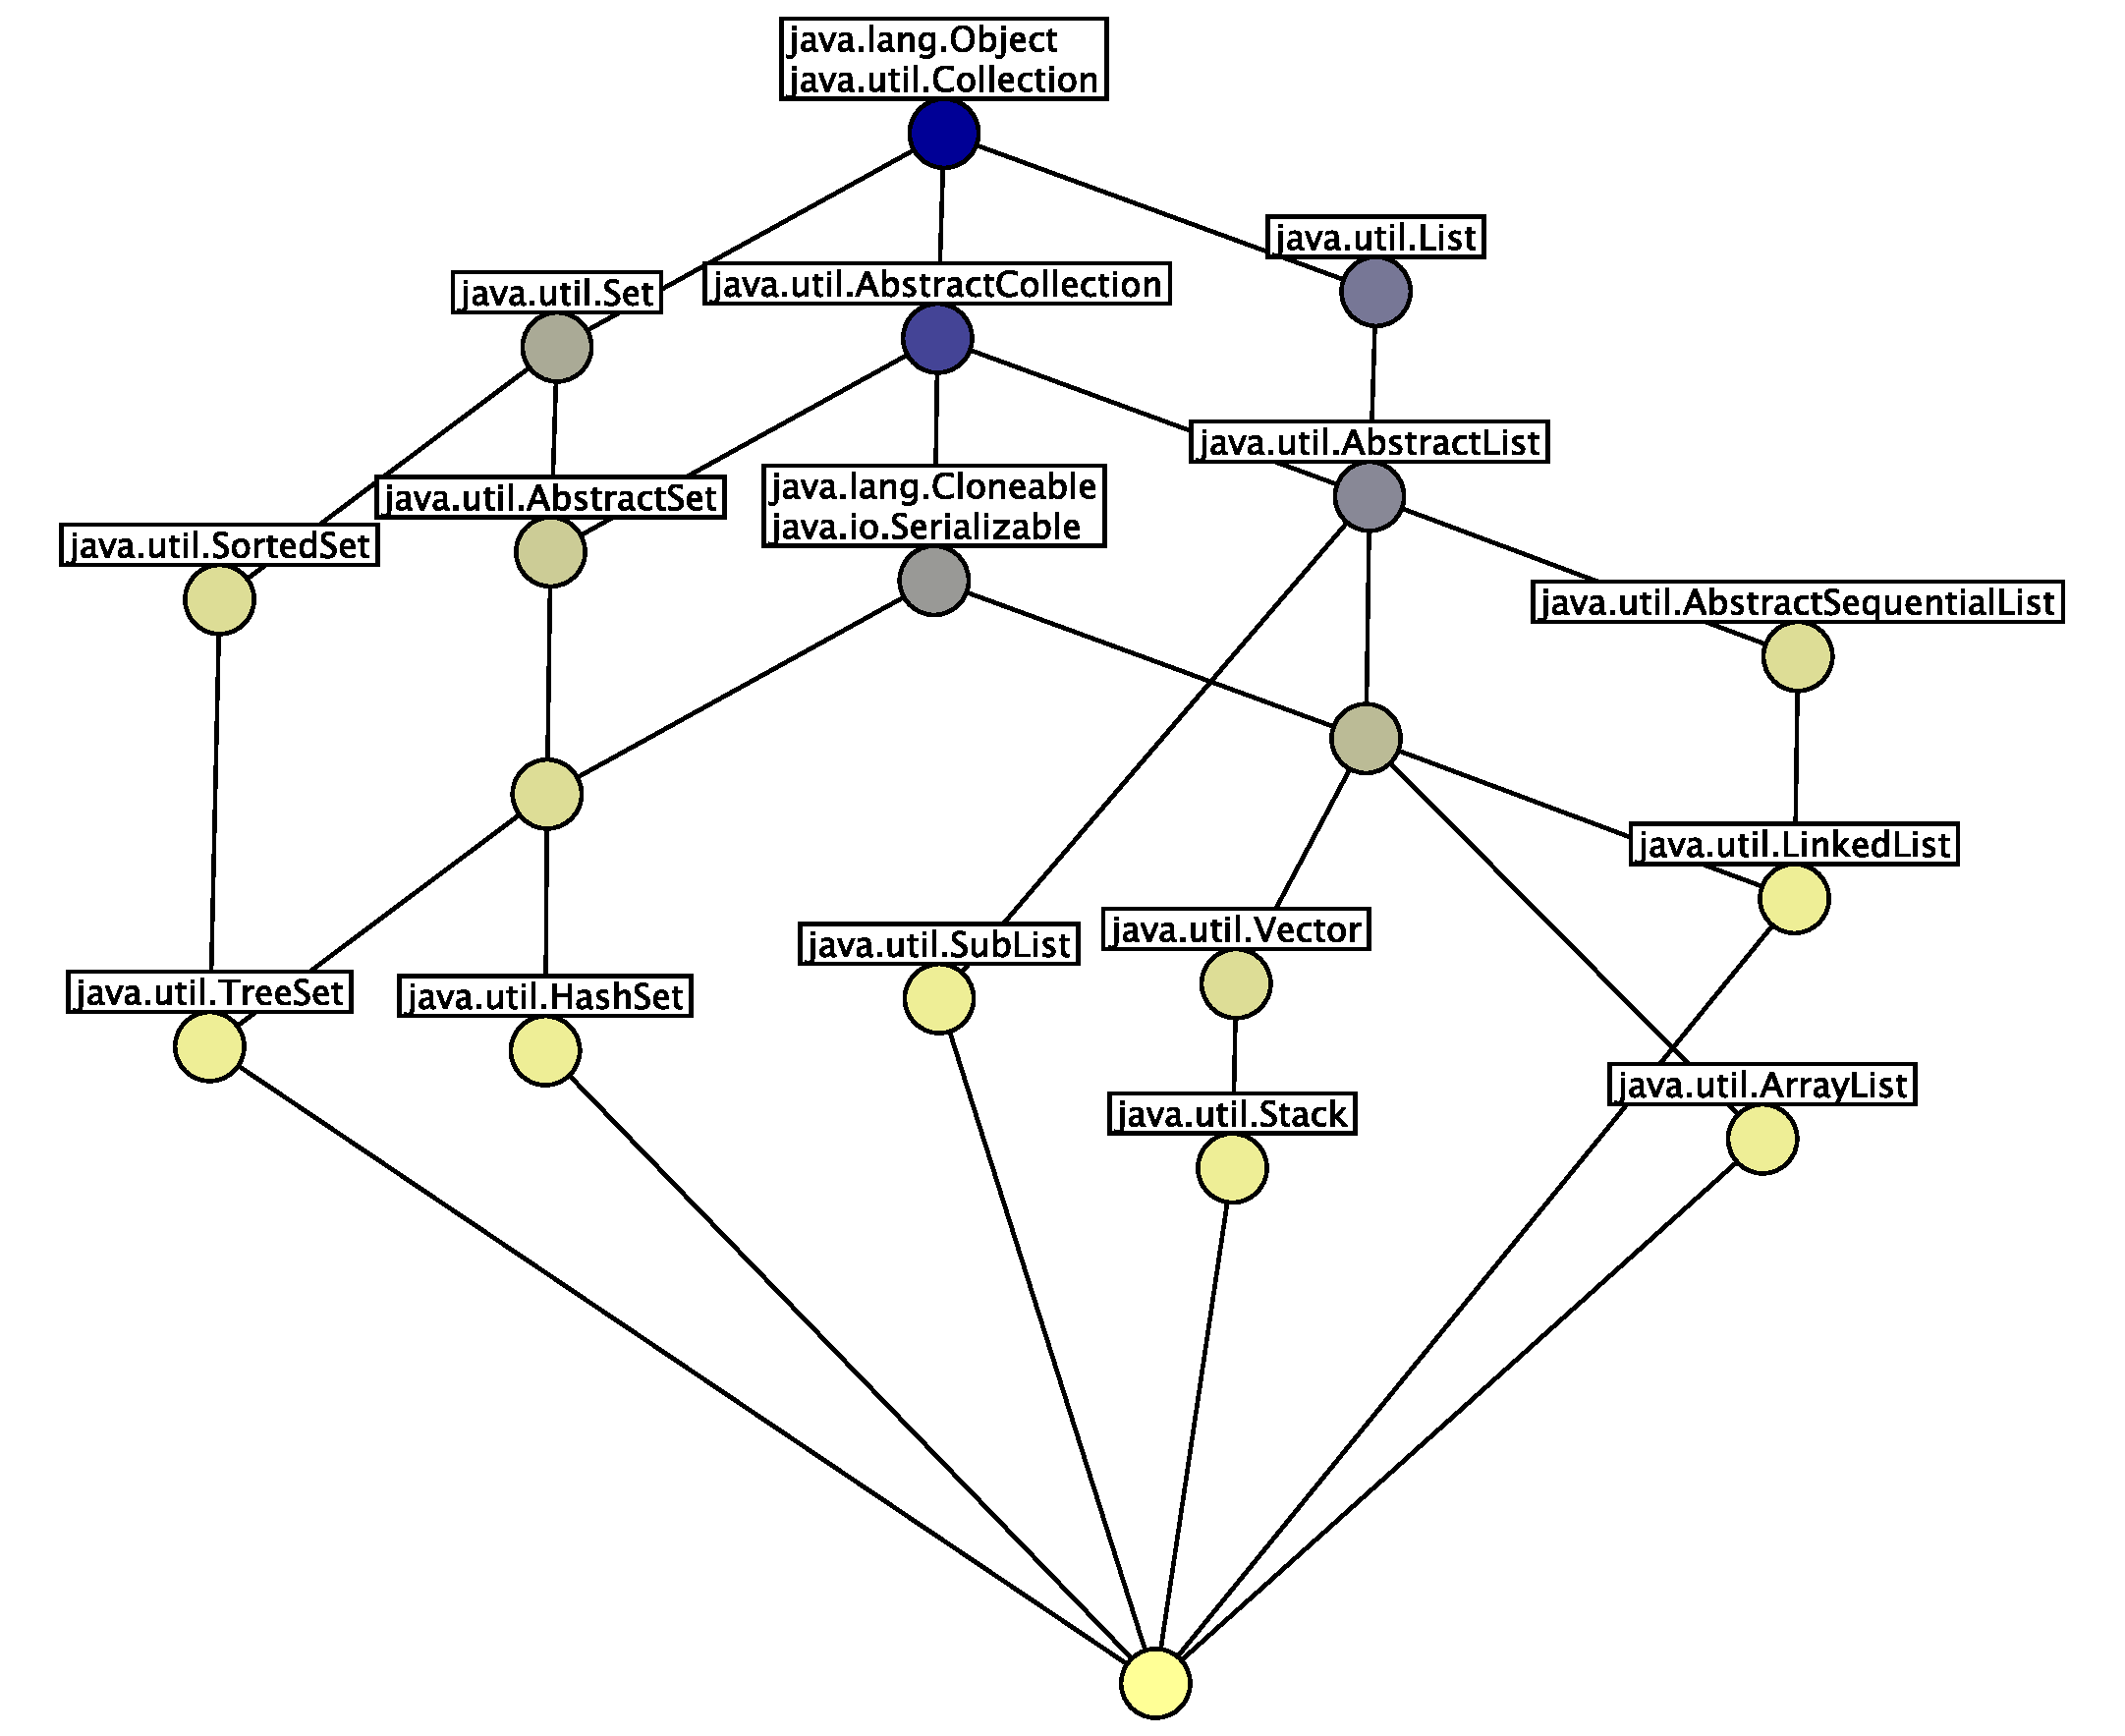
\includegraphics[height=0.8 \textheight]{img/class-hierarchy.eps}
 \end{center}
\end{slide}

\overlays{4}{
\begin{slide}{Decomposing the Collection API}
 \begin{center}
 \fromSlide{1}{%
  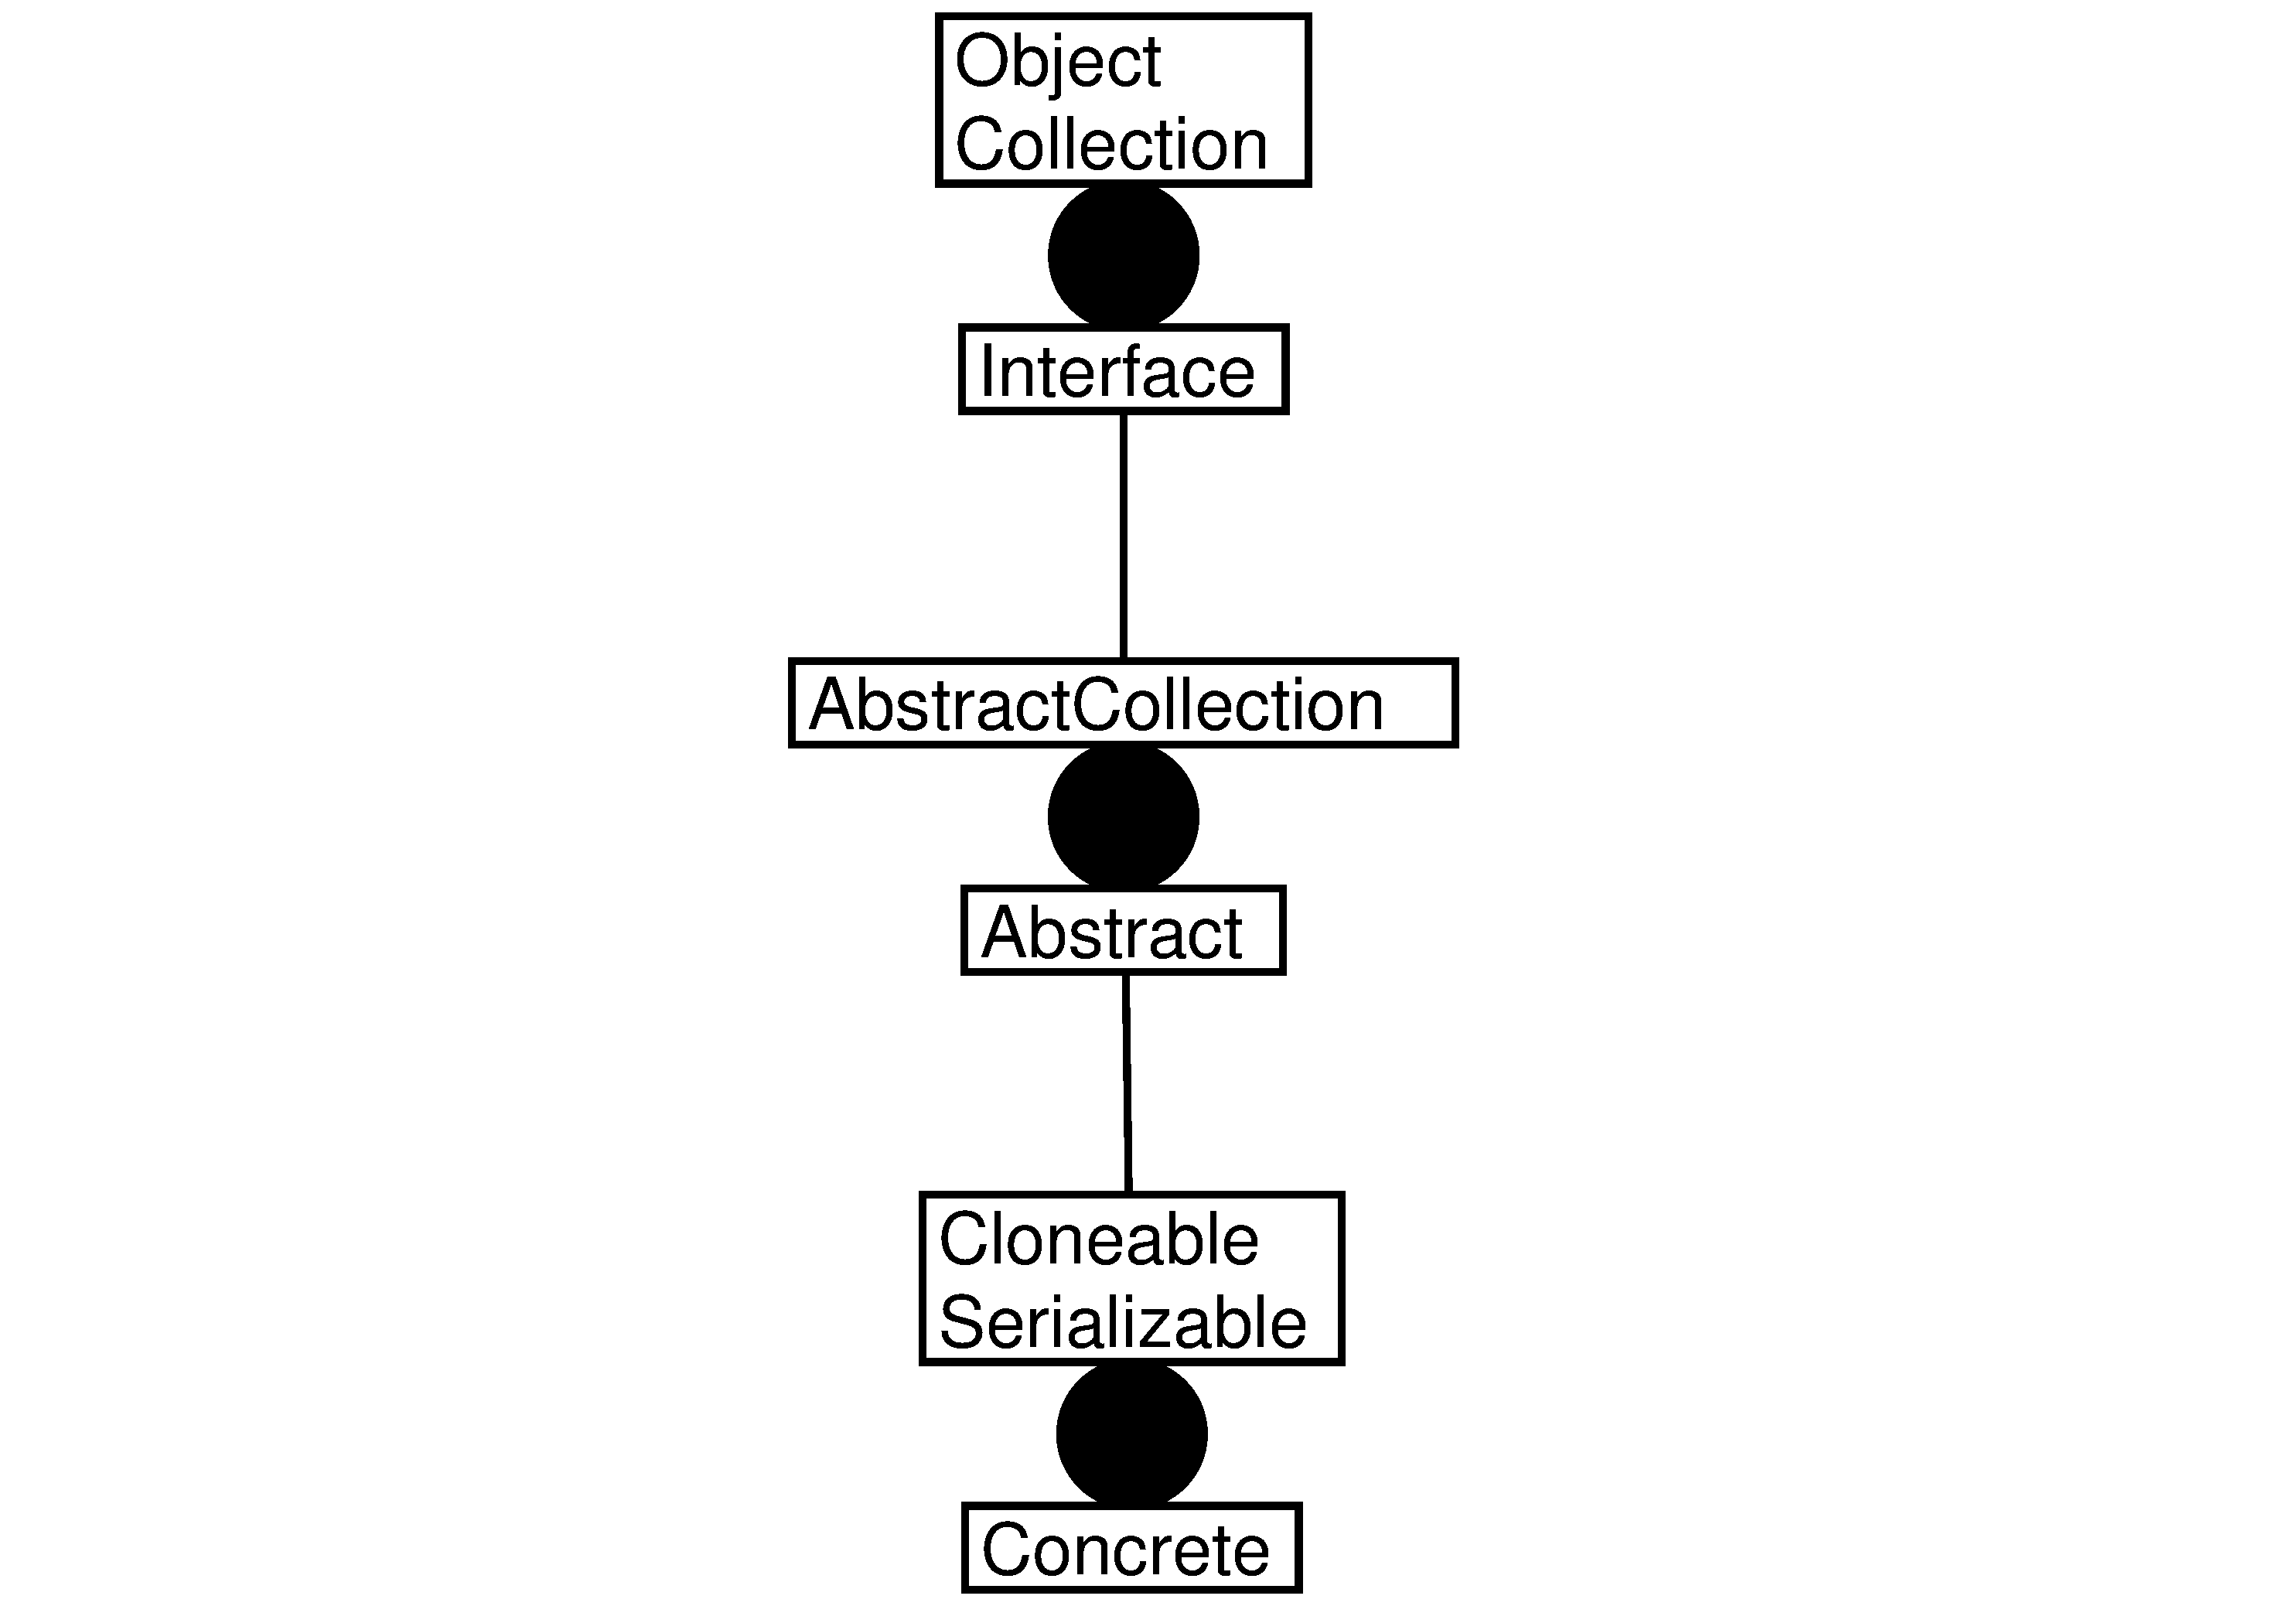
\includegraphics[height=0.3 \textheight]{img/jk1.eps}
 }%
 \fromSlide{2}{%
  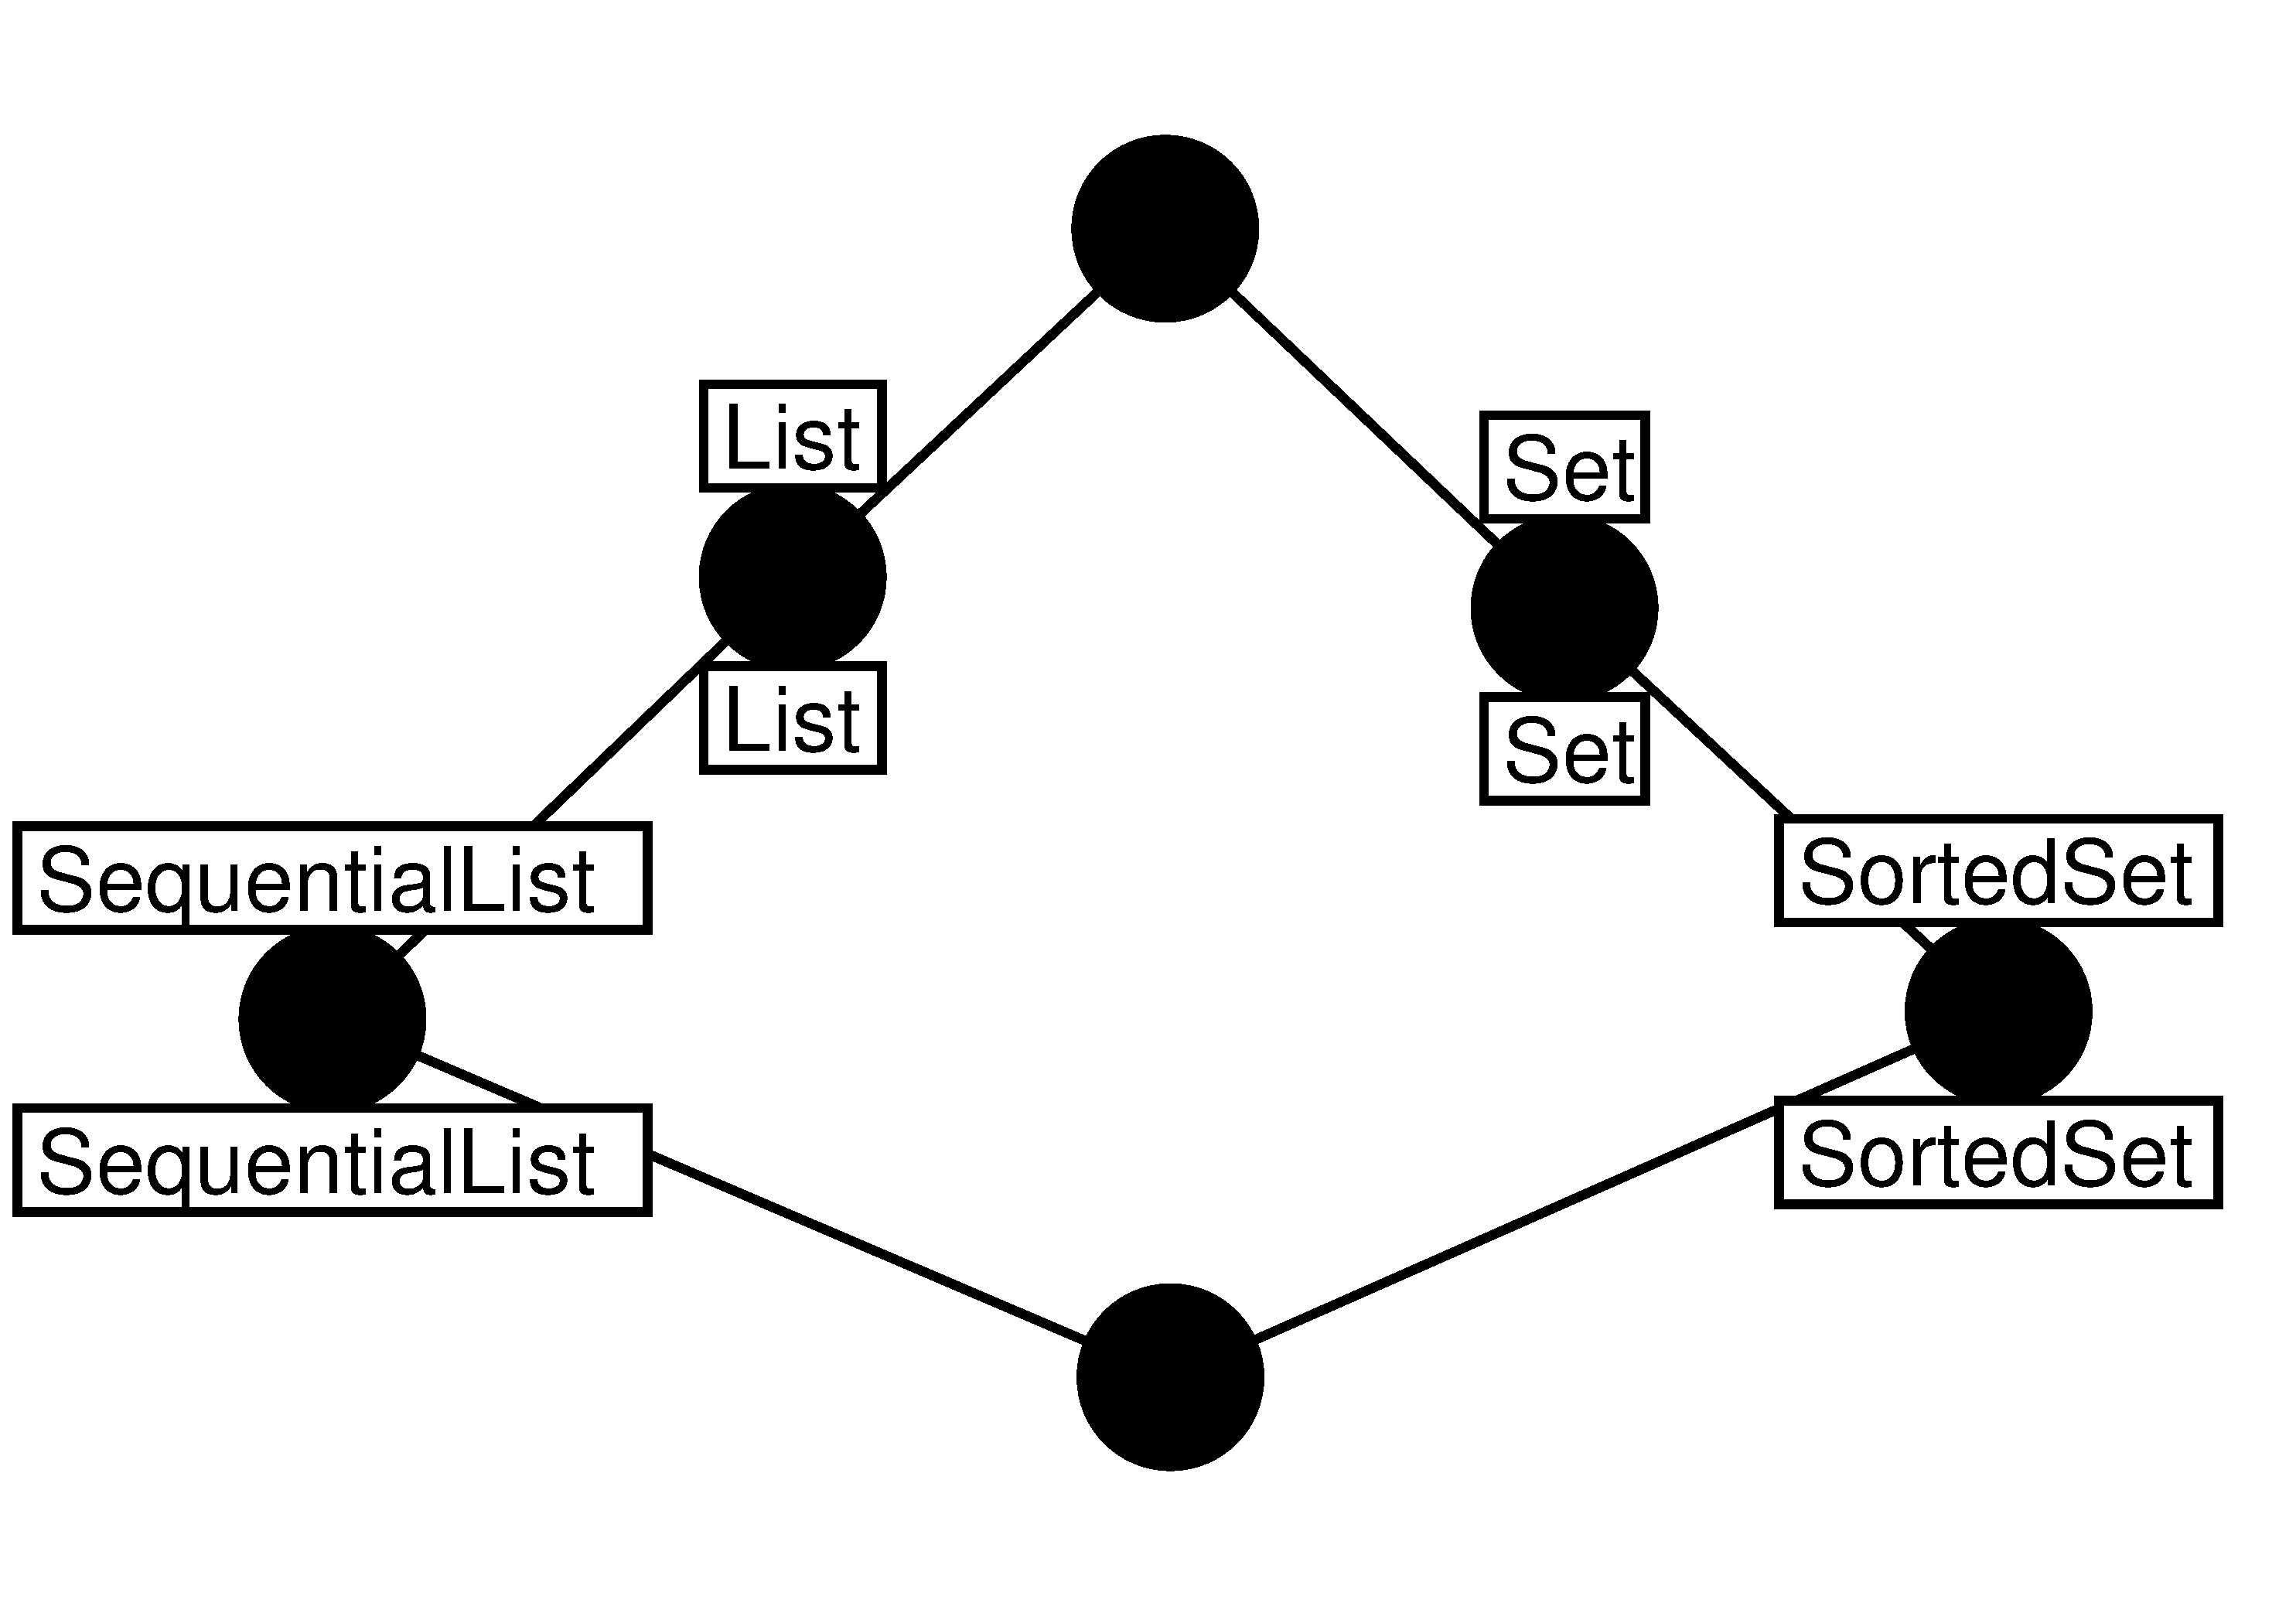
\includegraphics[height=0.3 \textheight]{img/jk2.eps} \\
 }%
 \fromSlide{3}{%
  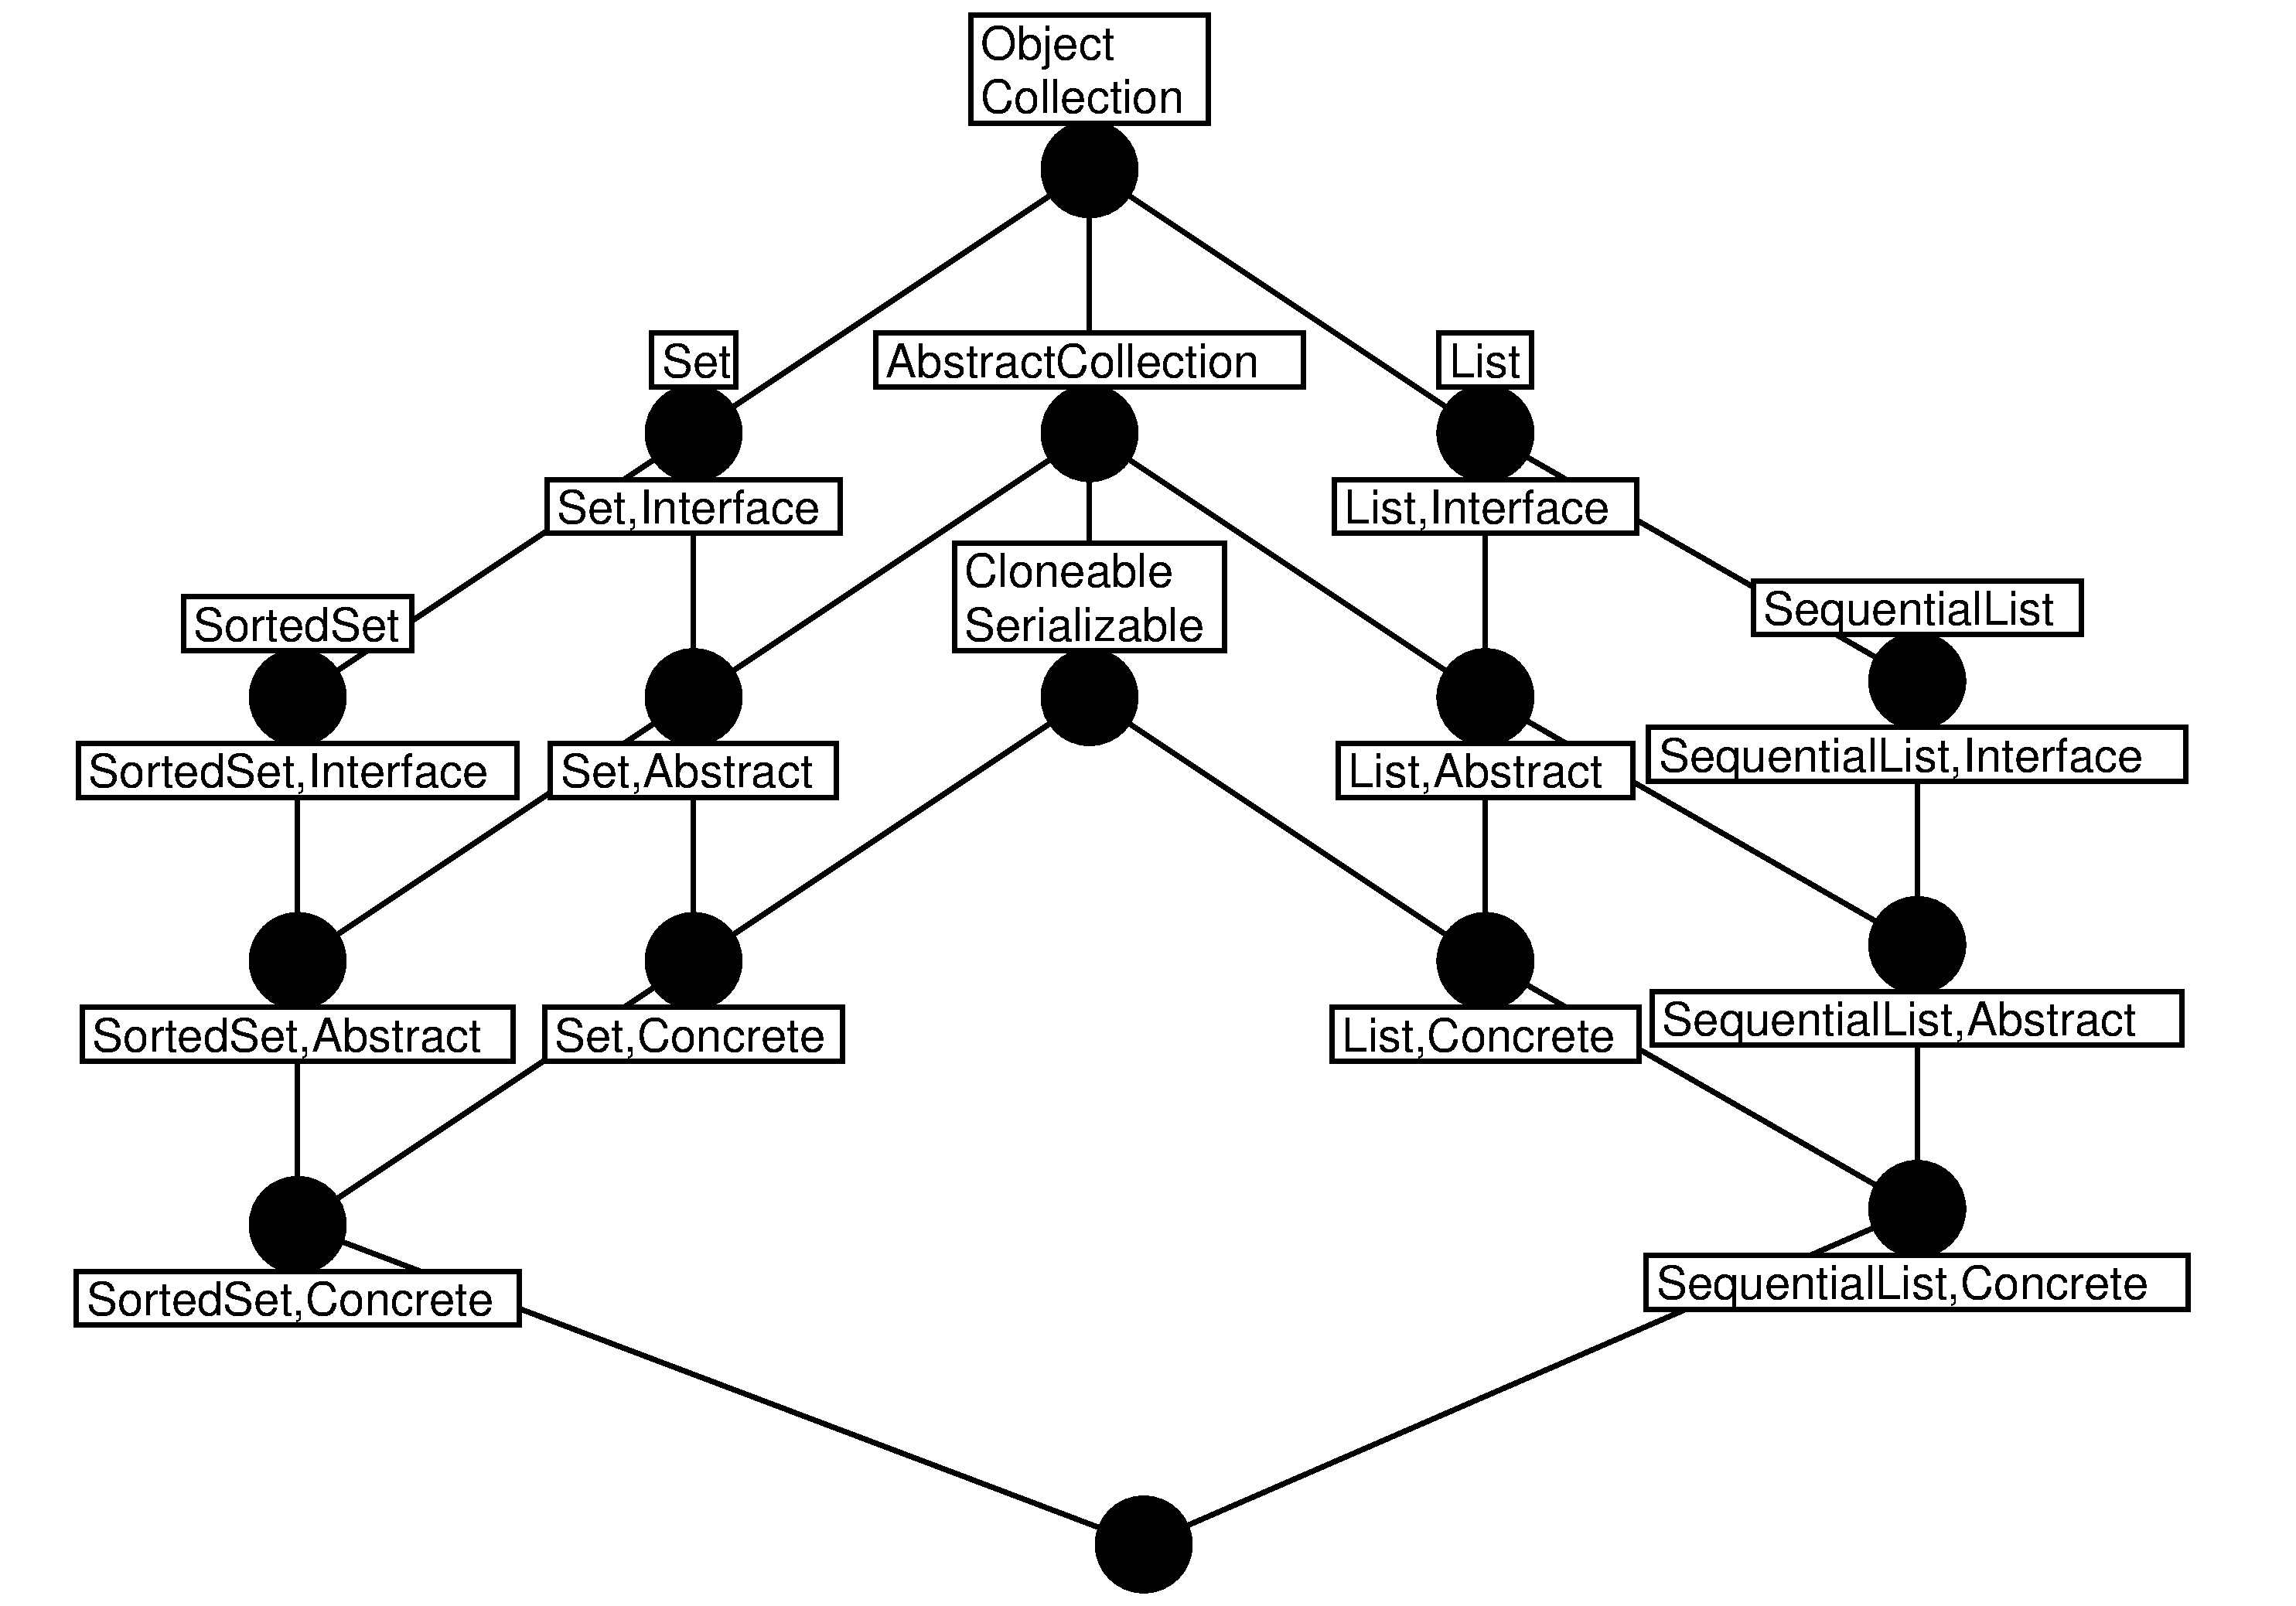
\includegraphics[width=0.4 \textwidth]{img/jk12.eps}
 }%
 \fromSlide{4}{%
  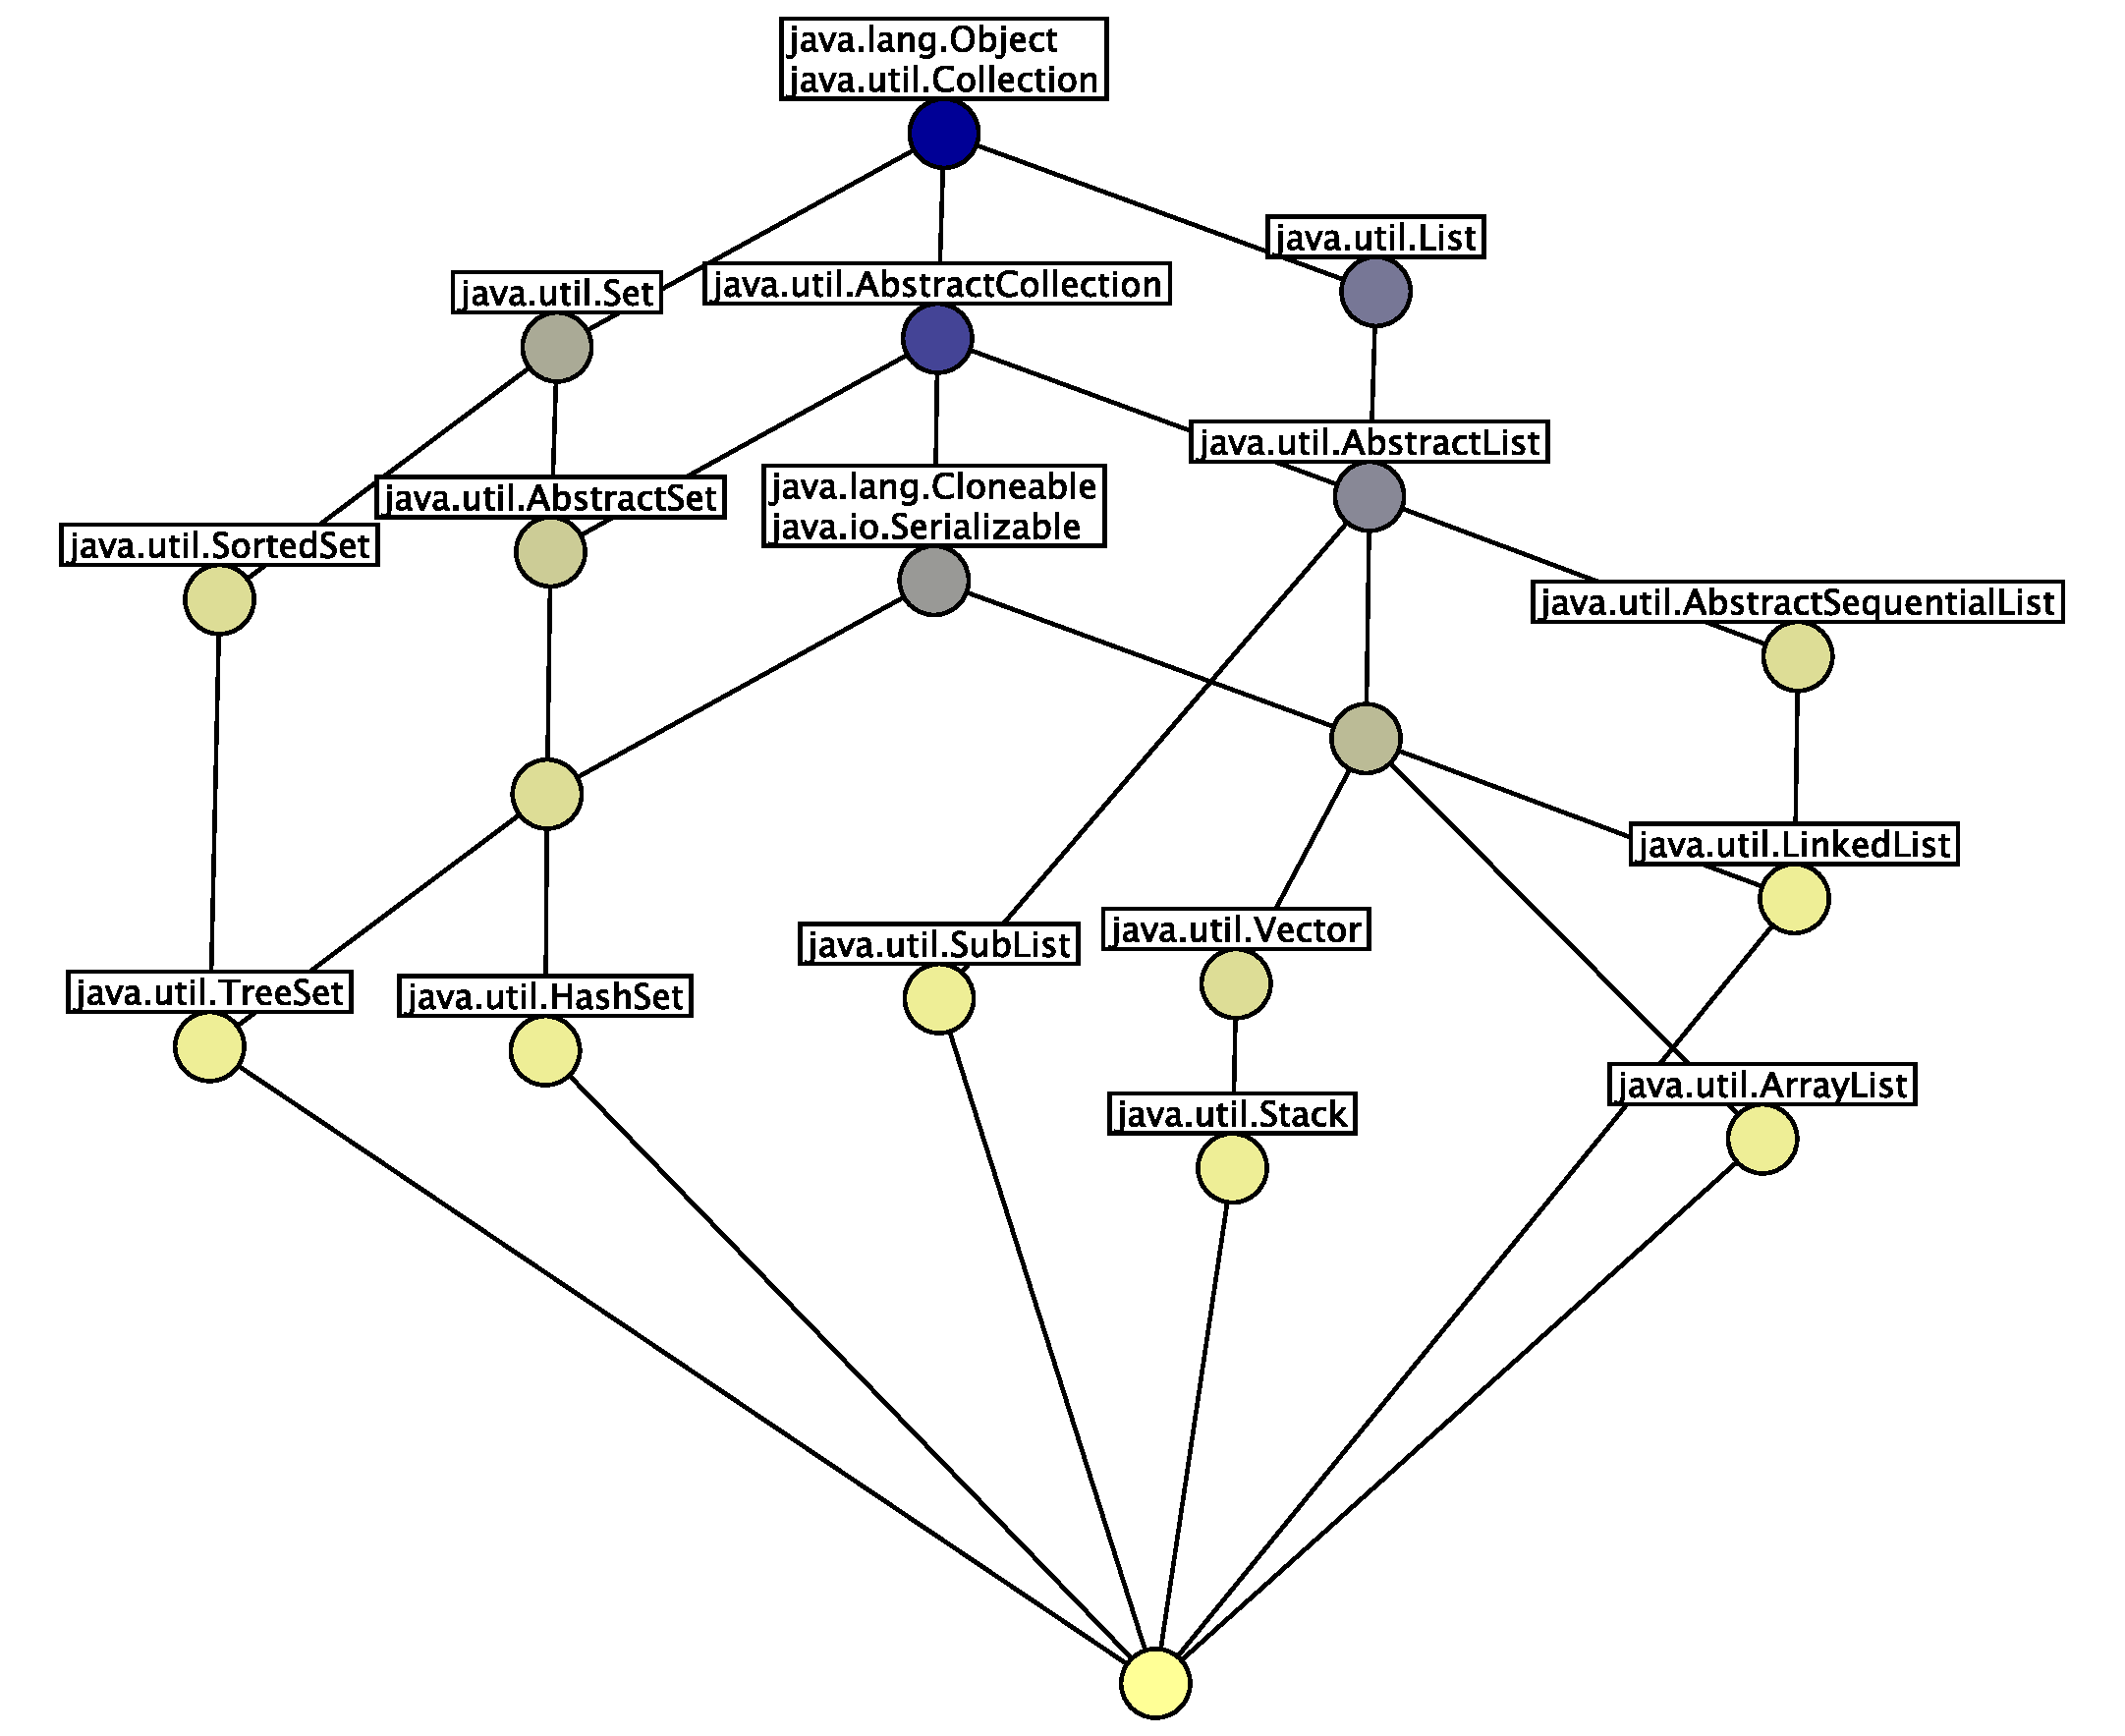
\includegraphics[width=0.4 \textwidth]{img/class-hierarchy.eps}
 }%
 \end{center}
\end{slide}
}

\part{Outlook}

\overlays{5}{
\begin{slide}{Technical Issues}
\begin{itemstep}
 \item Crepe is not integrated yet
 \item The other tools need better integration, too
 \item No UI for refining queries using the diagrams
 \item There will be bugs/glitches left
 \item Exploration currently limited to the ToscanaJ source code
       $\Rightarrow$ try CASS on various OSS Java projects
\end{itemstep}
\end{slide}
}

\overlays{5}{
\begin{slide}{Open Research Questions}
\begin{itemstep}
 \item Are there ways of using CASS that are helpful in most cases?
 \item What questions can be answered easily, which ones can't?
 \item How can the approach be used for automated testing?
 \item Can we include calling sequences in the analysis (e.g. \texttt{init()}
       must be called before other methods)?
 \item Can this be used to see changes over time? How would that be visualized?
\end{itemstep}
\end{slide}
}

\part{Thank you!}

\part{More examples}

\begin{slide}{Example: Jena toplevel view}
 \begin{center}
 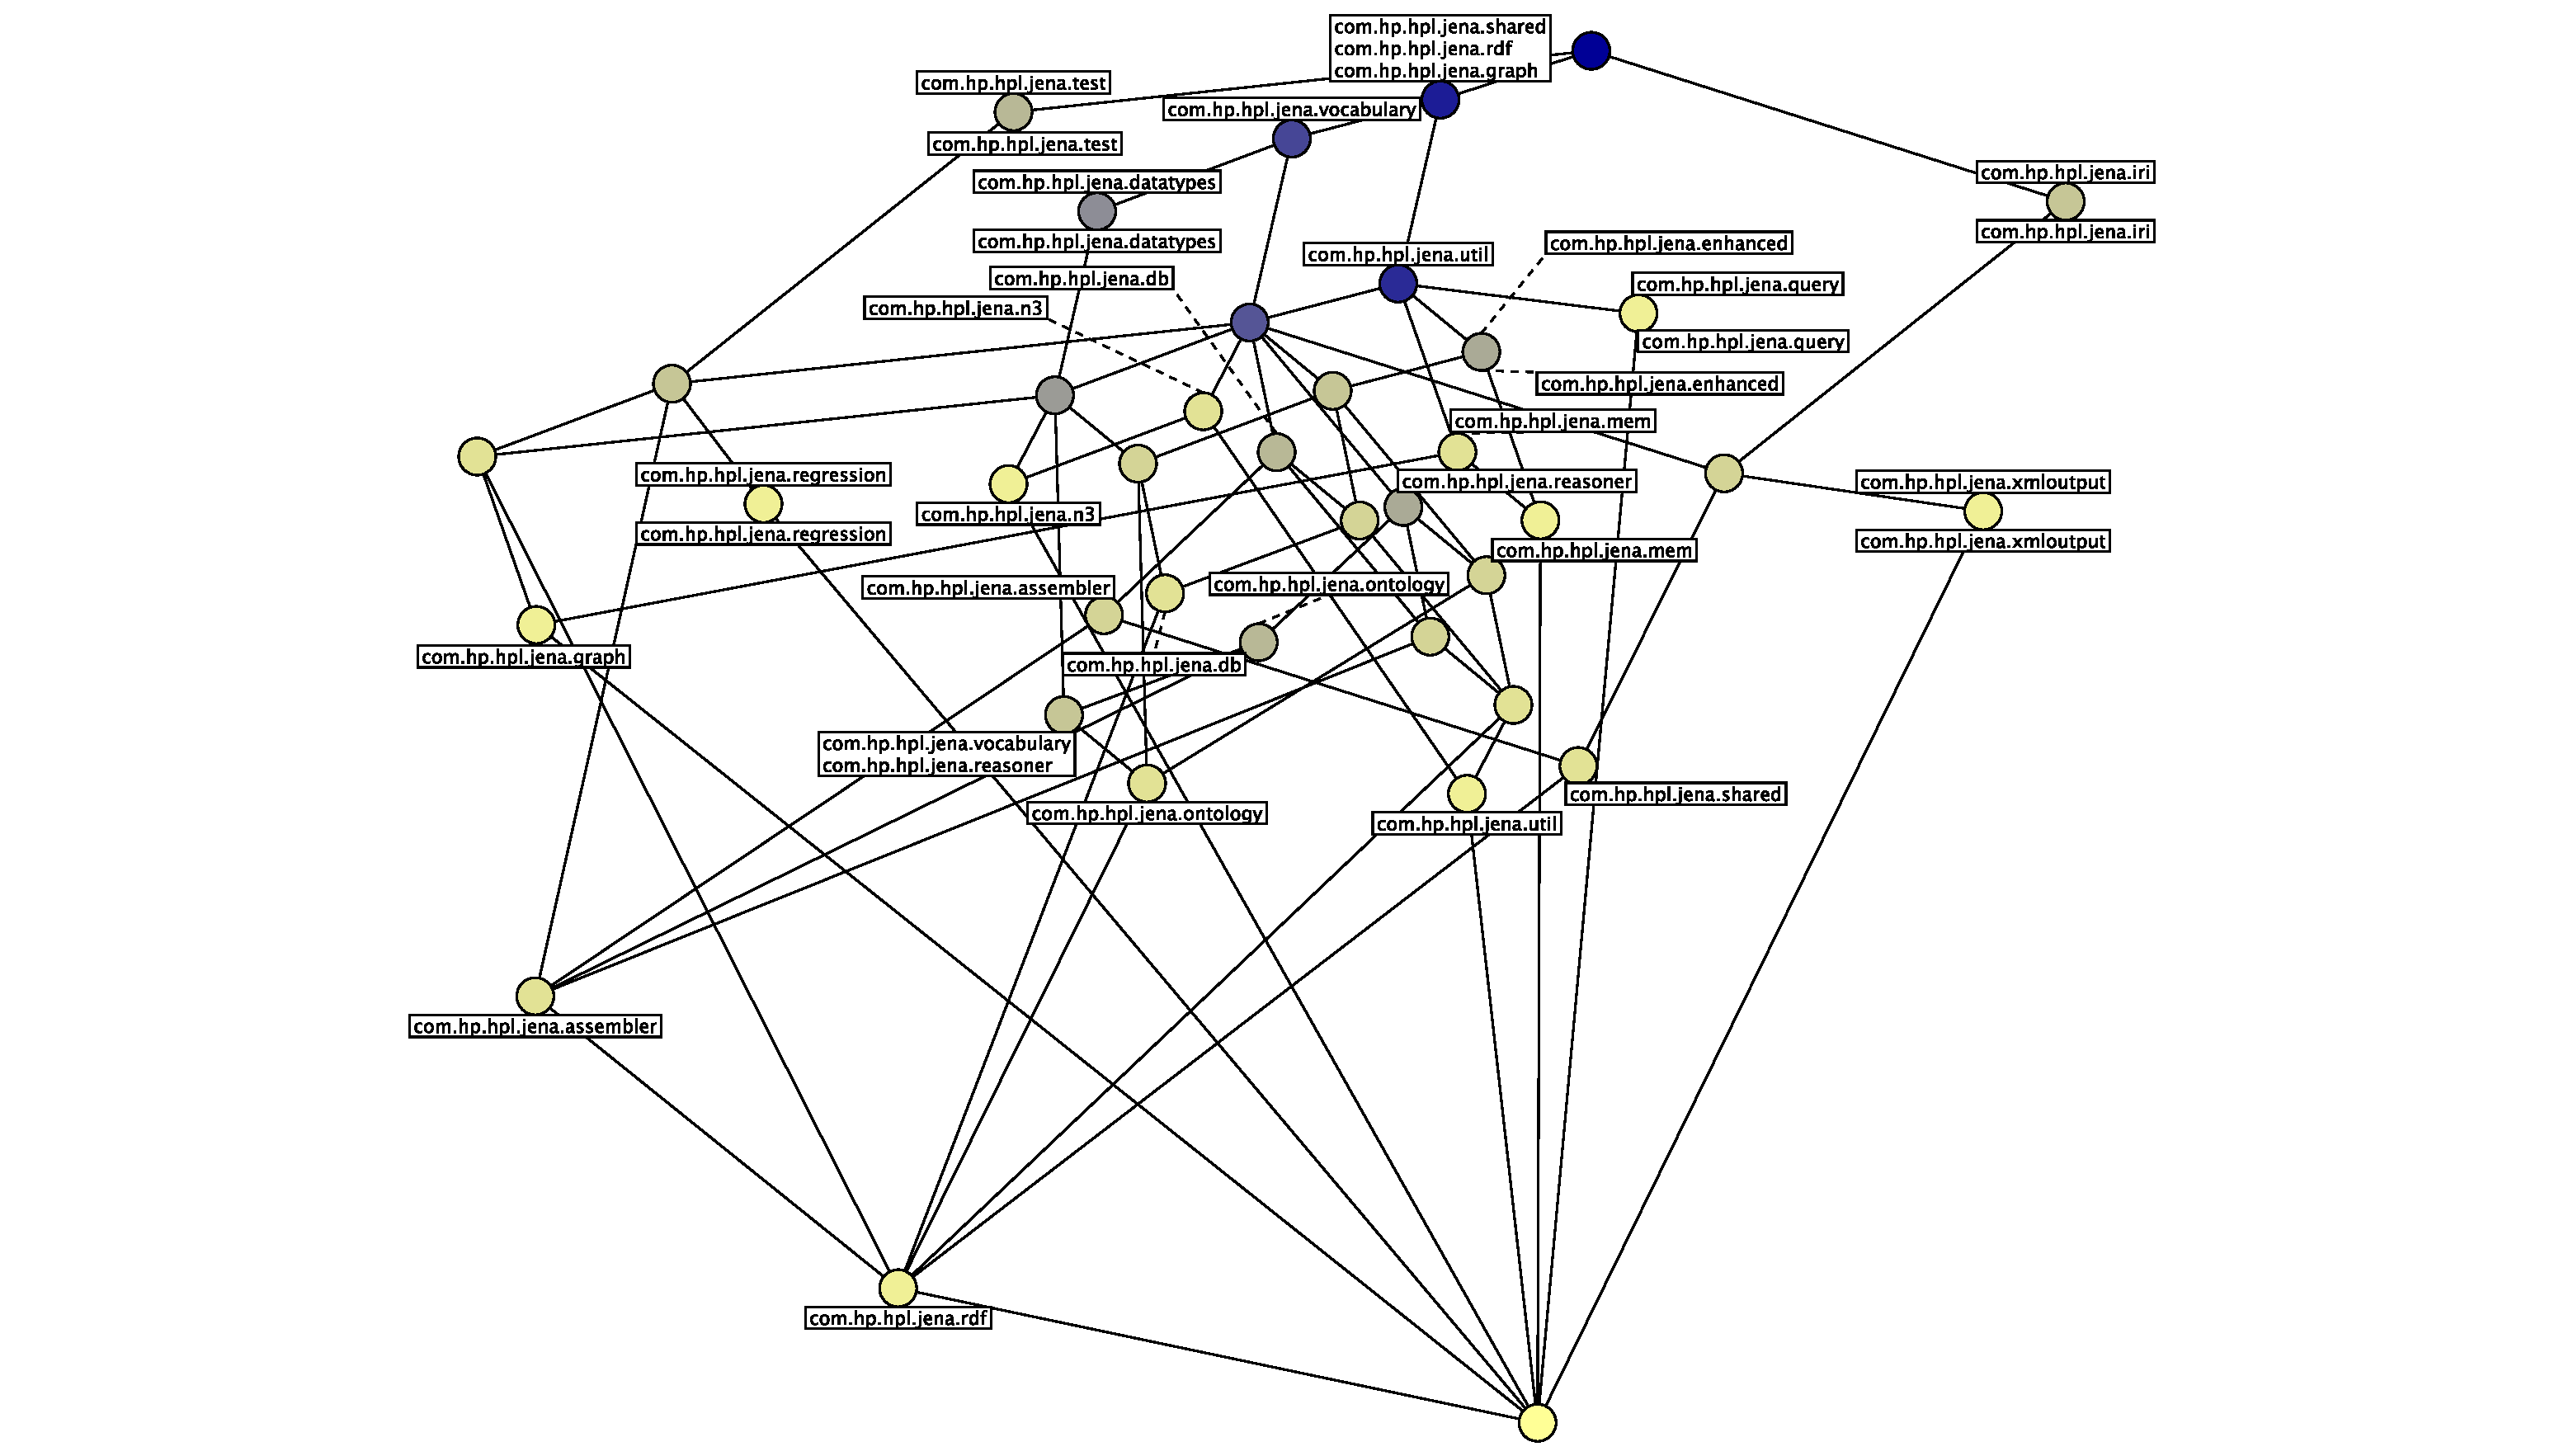
\includegraphics[width = \textwidth]{img/jenaToplevelDependencies.eps}
 % jenaToplevelDependencies.eps: 1x33 pixel, 300dpi, 0.01x0.28 cm, bb=20 239 575 552
\end{center}
\end{slide}

\begin{slide}{Example: small hierarchy}
 \begin{center}
 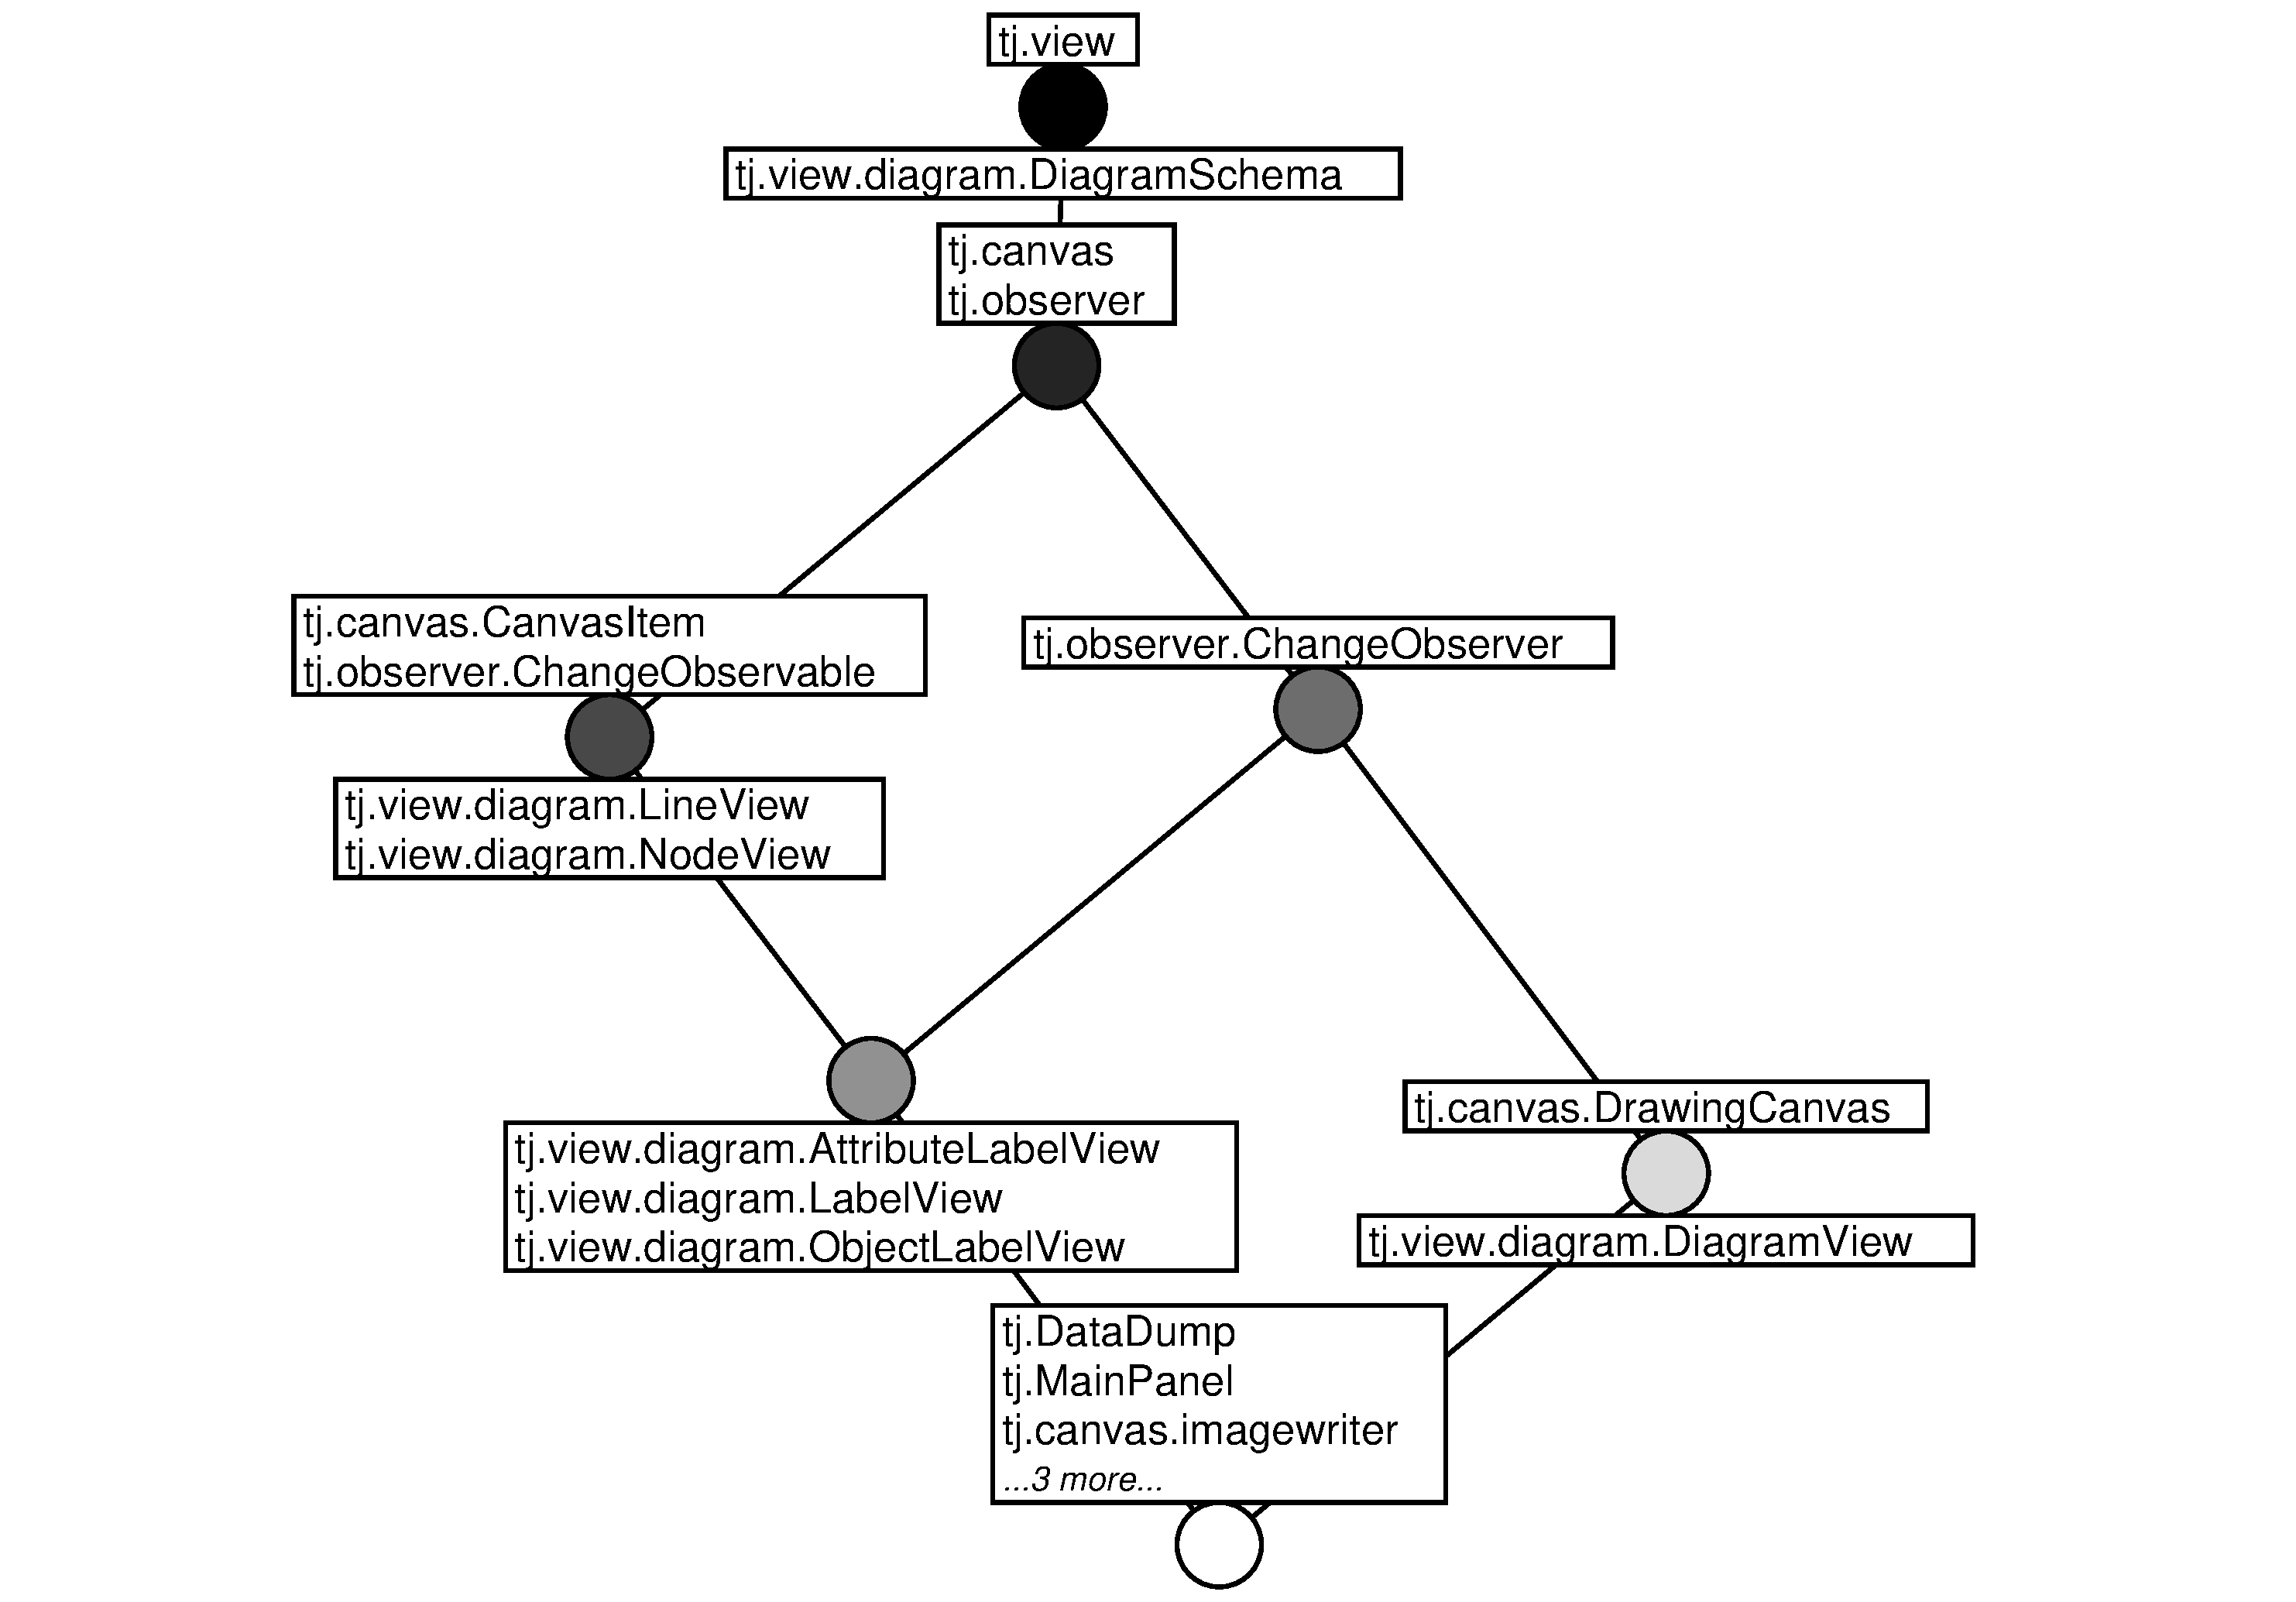
\includegraphics[height = 0.8 \textheight]{img/derives-4.eps}
\end{center}
\end{slide}

\end{document}

% templates
\ignore{

% slide with five items unfolding
\overlays{5}{
\begin{slide}{}
\begin{itemstep}
 \item 
 \item 
 \item 
 \item 
 \item 
\end{itemstep}
\end{slide}
}

% example graphic
\begin{slide}{Example: }
 \begin{center}
 \includegraphics[width = \textwidth]{img/.eps}
\end{center}
\end{slide}

}